%-----------------------------------------------------------------------------------------
% Autor dieser Vorlage:
% Stefan Macke (http://fachinformatiker-anwendungsentwicklung.net)
% Permalink zur Vorlage: http://fiae.link/LaTeXVorlageFIAE
%
% Sämtliche verwendeten Abbildungen, Tabellen und Listings stammen von Dirk Grashorn.
%
% Lizenz: Creative Commons 4.0 Namensnennung - Weitergabe unter gleichen Bedingungen
% -----------------------------------------------------------------------------------------

\documentclass[
	11pt,
	ngerman,
	toc=listof, % Abbildungsverzeichnis sowie Tabellenverzeichnis in das Inhaltsverzeichnis aufnehmen
	toc=bibliography, % Literaturverzeichnis in das Inhaltsverzeichnis aufnehmen
	footnotes=multiple, % Trennen von direkt aufeinander folgenden Fußnoten
	parskip=half, % vertikalen Abstand zwischen Absätzen verwenden anstatt horizontale Einrückung von Folgeabsätzen
	numbers=noendperiod % Den letzten Punkt nach einer Nummerierung entfernen (nach DIN 5008)
]{scrartcl}
\pdfminorversion=5 % erlaubt das Einfügen von pdf-Dateien bis Version 1.7, ohne eine Fehlermeldung zu werfen (keine Garantie für fehlerfreies Einbetten!)
\usepackage[utf8]{inputenc} % muss als erstes eingebunden werden, da Meta/Packages ggfs. Sonderzeichen enthalten

% !TEX root = Projektdokumentation.tex

% Hinweis: der Titel muss zum Inhalt des Projekts passen und den zentralen Inhalt des Projekts deutlich herausstellen
\newcommand{\titel}{ReklaTool}
\newcommand{\untertitel}{Entwicklung einer Webanwendung zur Abfrage und Anzeige\\ 
von Kalkulationsvorgängen aus dem Kfz-Bereich \\nach dem Client-Server-Prinzip}
\newcommand{\kompletterTitel}{\titel{} -- \untertitel}

\newcommand{\autorName}{Ingolf Schieck}
\newcommand{\autorAnschrift}{Hähnelstraße 21}
\newcommand{\autorOrt}{04177 Leipzig}
\newcommand{\autorId}{661537}


\newcommand{\betriebLogo}{ICAM-logo.png}
\newcommand{\betriebName}{IcamSystems GmbH}
\newcommand{\betriebAnschrift}{Käthe-Kollwitz-Straße 84}
\newcommand{\betriebOrt}{04109 Leipzig}

\newcommand{\ausbildungsberuf}{Fachinformatiker/Fachinformatikerin (VO 2020) Fachrichtung:
Anwendungsentwicklung, Leipzig FIAE 4 (AP T2V1)}
\newcommand{\betreff}{Dokumentation zur betrieblichen Projektarbeit}
\newcommand{\pruefungstermin}{Winter 2022}
\newcommand{\abgabeOrt}{Leipzig}
\newcommand{\abgabeTermin}{23.11.2022}
 % Metadaten zu diesem Dokument (Autor usw.)
% !TEX root = ../Projektdokumentation.tex

% Anpassung an Landessprache ---------------------------------------------------
\usepackage{babel}

% Umlaute ----------------------------------------------------------------------
%   Umlaute/Sonderzeichen wie äüöß direkt im Quelltext verwenden (CodePage).
%   Erlaubt automatische Trennung von Worten mit Umlauten.
% ------------------------------------------------------------------------------
\usepackage[T1]{fontenc}
\usepackage{textcomp} % Euro-Zeichen etc.

% Schrift ----------------------------------------------------------------------
\usepackage{lmodern} % bessere Fonts
\usepackage{relsize} % Schriftgröße relativ festlegen

% Tabellen ---------------------------------------------------------------------
\PassOptionsToPackage{table}{xcolor}
\usepackage{tabularx}
\usepackage{booktabs}
% für lange Tabellen
\usepackage{longtable}
\usepackage{array}
\usepackage{ragged2e}
\usepackage{lscape}
\newcolumntype{w}[1]{>{\raggedleft\hspace{0pt}}p{#1}} % Spaltendefinition rechtsbündig mit definierter Breite

% Grafiken ---------------------------------------------------------------------
\usepackage[dvips,final]{graphicx} % Einbinden von JPG-Grafiken ermöglichen
\usepackage{graphics} % keepaspectratio
\usepackage{floatflt} % zum Umfließen von Bildern
\graphicspath{{Bilder/}} % hier liegen die Bilder des Dokuments

% Sonstiges --------------------------------------------------------------------
\usepackage[titles]{tocloft} % Inhaltsverzeichnis DIN 5008 gerecht einrücken
\usepackage{amsmath,amsfonts} % Befehle aus AMSTeX für mathematische Symbole
\usepackage{enumitem} % anpassbare Enumerates/Itemizes
\usepackage{xspace} % sorgt dafür, dass Leerzeichen hinter parameterlosen Makros nicht als Makroendezeichen interpretiert werden

\usepackage{makeidx} % für Index-Ausgabe mit \printindex
\usepackage[printonlyused]{acronym} % es werden nur benutzte Definitionen aufgelistet

% Einfache Definition der Zeilenabstände und Seitenränder etc.
\usepackage{setspace}
\usepackage{geometry}

% Symbolverzeichnis
\usepackage[intoc]{nomencl}
\let\abbrev\nomenclature
\renewcommand{\nomname}{Abkürzungsverzeichnis}
\setlength{\nomlabelwidth}{.25\hsize}
\renewcommand{\nomlabel}[1]{#1 \dotfill}
\setlength{\nomitemsep}{-\parsep}

\usepackage{varioref} % Elegantere Verweise. „auf der nächsten Seite“
\usepackage{url} % URL verlinken, lange URLs umbrechen etc.

\usepackage{chngcntr} % fortlaufendes Durchnummerieren der Fußnoten
% \usepackage[perpage]{footmisc} % Alternative: Nummerierung der Fußnoten auf jeder Seite neu

\usepackage{ifthen} % bei der Definition eigener Befehle benötigt
\usepackage{todonotes} % definiert u.a. die Befehle \todo und \listoftodos
\usepackage[square]{natbib} % wichtig für korrekte Zitierweise

% PDF-Optionen -----------------------------------------------------------------
\usepackage{pdfpages}
\pdfminorversion=5 % erlaubt das Einfügen von pdf-Dateien bis Version 1.7, ohne eine Fehlermeldung zu werfen (keine Garantie für fehlerfreies Einbetten!)
\usepackage[
    bookmarks,
    bookmarksnumbered,
    bookmarksopen=true,
    bookmarksopenlevel=1,
    colorlinks=true,
% diese Farbdefinitionen zeichnen Links im PDF farblich aus
    anchorcolor=AOBlau,% Ankertext
    citecolor=AOBlau, % Verweise auf Literaturverzeichniseinträge im Text
    filecolor=AOBlau, % Verknüpfungen, die lokale Dateien öffnen
    menucolor=AOBlau, % Acrobat-Menüpunkte
    urlcolor=AOBlau,
% diese Farbdefinitionen sollten für den Druck verwendet werden (alles schwarz)
    %linkcolor=black, % einfache interne Verknüpfungen
    %anchorcolor=black, % Ankertext
    %citecolor=black, % Verweise auf Literaturverzeichniseinträge im Text
    %filecolor=black, % Verknüpfungen, die lokale Dateien öffnen
    %menucolor=black, % Acrobat-Menüpunkte
    %urlcolor=black,
%
    %backref, % Quellen werden zurück auf ihre Zitate verlinkt
    pdftex,
    plainpages=false, % zur korrekten Erstellung der Bookmarks
    pdfpagelabels=true, % zur korrekten Erstellung der Bookmarks
    hypertexnames=false, % zur korrekten Erstellung der Bookmarks
    linkcolor=black,
    linktoc=all,
]{hyperref}
% Befehle, die Umlaute ausgeben, führen zu Fehlern, wenn sie hyperref als Optionen übergeben werden
\hypersetup{
    pdftitle={\titel -- \untertitel},
    pdfauthor={\autorName},
    pdfcreator={\autorName},
    pdfsubject={\titel -- \untertitel},
    pdfkeywords={\titel -- \untertitel},
}


% zum Einbinden von Programmcode -----------------------------------------------
\usepackage{listings}
\usepackage{xcolor}
\definecolor{hellgelb}{rgb}{1,1,0.9}
\definecolor{colKeys}{rgb}{0,0,1}
\definecolor{colIdentifier}{rgb}{0,0,0}
\definecolor{colComments}{rgb}{0,0.5,0}
\definecolor{colString}{rgb}{1,0,0}
\lstset{
    float=hbp,
	basicstyle=\footnotesize,
    identifierstyle=\color{colIdentifier},
    keywordstyle=\color{colKeys},
    stringstyle=\color{colString},
    commentstyle=\color{colComments},
    backgroundcolor=\color{hellgelb},
    columns=flexible,
    tabsize=2,
    frame=single,
    extendedchars=true,
    showspaces=false,
    showstringspaces=false,
    numbers=left,
    numberstyle=\tiny,
    breaklines=true,
    breakautoindent=true,
	captionpos=b,
}
\lstdefinelanguage{cs}{
	sensitive=false,
	morecomment=[l]{//},
	morecomment=[s]{/*}{*/},
	morestring=[b]",
	morekeywords={
		abstract,event,new,struct,as,explicit,null,switch
		base,extern,object,this,bool,false,operator,throw,
		break,finally,out,true,byte,fixed,override,try,
		case,float,params,typeof,catch,for,private,uint,
		char,foreach,protected,ulong,checked,goto,public,unchecked,
		class,if,readonly,unsafe,const,implicit,ref,ushort,
		continue,in,return,using,decimal,int,sbyte,virtual,
		default,interface,sealed,volatile,delegate,internal,short,void,
		do,is,sizeof,while,double,lock,stackalloc,
		else,long,static,enum,namespace,string},
}
\lstdefinelanguage{natural}{
	sensitive=false,
	morecomment=[l]{/*},
	morestring=[b]",
	morestring=[b]',
	alsodigit={-,*},
	morekeywords={
		DEFINE,DATA,LOCAL,END-DEFINE,WRITE,CALLNAT,PARAMETER,USING,
		IF,NOT,END-IF,ON,*ERROR-NR,ERROR,END-ERROR,ESCAPE,ROUTINE,
		PERFORM,SUBROUTINE,END-SUBROUTINE,CONST,END-FOR,END,FOR,RESIZE,
		ARRAY,TO,BY,VALUE,RESET,COMPRESS,INTO,EQ},
}
\lstdefinelanguage{php}{
	sensitive=false,
	morecomment=[l]{/*},
	morestring=[b]",
	morestring=[b]',
	alsodigit={-,*},
	morekeywords={
		abstract,and,array,as,break,case,catch,cfunction,class,clone,const,
		continue,declare,default,do,else,elseif,enddeclare,endfor,endforeach,
		endif,endswitch,endwhile,extends,final,for,foreach,function,global,
		goto,if,implements,interface,instanceof,namespace,new,old_function,or,
		private,protected,public,static,switch,throw,try,use,var,while,xor
		die,echo,empty,exit,eval,include,include_once,isset,list,require,
		require_once,return,print,unset},
}
 % verwendete Packages
% !TEX root = ../Projektdokumentation.tex

% Seitenränder -----------------------------------------------------------------
\setlength{\topskip}{\ht\strutbox} % behebt Warnung von geometry
\geometry{a3paper,landscape,left=25mm,right=25mm,top=25mm,bottom=35mm}

\usepackage[
	automark, % Kapitelangaben in Kopfzeile automatisch erstellen
	headsepline, % Trennlinie unter Kopfzeile
	ilines % Trennlinie linksbündig ausrichten
]{scrlayer-scrpage}

% Kopf- und Fußzeilen ----------------------------------------------------------
\pagestyle{scrheadings}
% chapterpagestyle gibt es nicht in scrartcl
%\renewcommand{\chapterpagestyle}{scrheadings}
\clearscrheadfoot

% Kopfzeile
\renewcommand{\headfont}{\normalfont} % Schriftform der Kopfzeile
\ihead{\large{\textsc{\titel}}\\ \small{\untertitel} \\[1.5ex] \textit{\headmark}}
\chead{}
\ohead{\includegraphics[scale=0.2]{\betriebLogo}}
\setlength{\headheight}{20mm} % Höhe der Kopfzeile
%\setheadwidth[0pt]{textwithmarginpar} % Kopfzeile über den Text hinaus verbreitern (falls Logo den Text überdeckt)

% Fußzeile
\ifoot{\autorName}
\cfoot{Identnummer: \autorId}
\ofoot{\pagemark}

% Überschriften nach DIN 5008 in einer Fluchtlinie
% ------------------------------------------------------------------------------

% Abstand zwischen Nummerierung und Überschrift definieren
% > Schön wäre hier die dynamische Berechnung des Abstandes in Abhängigkeit
% > der Verschachtelungstiefe des Inhaltsverzeichnisses
\newcommand{\headingSpace}{1.5cm}

% Abschnittsüberschriften im selben Stil wie beim Inhaltsverzeichnis einrücken
\renewcommand*{\othersectionlevelsformat}[3]{
  \makebox[\headingSpace][l]{#3\autodot}
}

% Für die Einrückung wird das Paket tocloft benötigt
%\cftsetindents{chapter}{0.0cm}{\headingSpace}
\cftsetindents{section}{0.0cm}{\headingSpace}
\cftsetindents{subsection}{0.0cm}{\headingSpace}
\cftsetindents{subsubsection}{0.0cm}{\headingSpace}
\cftsetindents{figure}{0.0cm}{\headingSpace}
\cftsetindents{table}{0.0cm}{\headingSpace}


% Allgemeines
% ------------------------------------------------------------------------------

\onehalfspacing % Zeilenabstand 1,5 Zeilen
\frenchspacing % erzeugt ein wenig mehr Platz hinter einem Punkt

% Schusterjungen und Hurenkinder vermeiden
\clubpenalty = 10000
\widowpenalty = 10000
\displaywidowpenalty = 10000

% Quellcode-Ausgabe formatieren
\lstset{numbers=left, numberstyle=\tiny, numbersep=5pt, breaklines=true}
\lstset{emph={square}, emphstyle=\color{red}, emph={[2]root,base}, emphstyle={[2]\color{blue}}}

\counterwithout{footnote}{section} % Fußnoten fortlaufend durchnummerieren
\setcounter{tocdepth}{3} % im Inhaltsverzeichnis werden die Kapitel bis zum Level der subsubsection übernommen
\setcounter{secnumdepth}{3} % Kapitel bis zum Level der subsubsection werden nummeriert

% Aufzählungen anpassen
\renewcommand{\labelenumi}{\arabic{enumi}.}
\renewcommand{\labelenumii}{\arabic{enumi}.\arabic{enumii}.}
\renewcommand{\labelenumiii}{\arabic{enumi}.\arabic{enumii}.\arabic{enumiii}}

% Tabellenfärbung:
\definecolor{heading}{rgb}{0.36,0.82,0.42}
\definecolor{odd}{rgb}{0.9,0.9,0.9}
 % Definitionen zum Aussehen der Seiten
% Abkürzungen
\newcommand{\Versis}{\textsc{Versis}\xspace}
\newcommand{\NI}{NatInfo\xspace}
\newcommand{\AO}{\textsc{Alte Oldenburger} Krankenversicherung\xspace}
 % eigene allgemeine Befehle, die z.B. die Arbeit mit LaTeX erleichtern
% Abkürzungen
\newcommand{\Versis}{\textsc{Versis}\xspace}
\newcommand{\NI}{NatInfo\xspace}
\newcommand{\AO}{\textsc{Alte Oldenburger} Krankenversicherung\xspace}
 % eigene projektspezifische Befehle, z.B. Abkürzungen usw.

\begin{document}

% kann nach dem Lesen entfernt werden ---------------------------------------
%\pagestyle{plain}
%% !TEX root = Projektdokumentation.tex
\section*{Über diese Vorlage}

Diese \LaTeX-Vorlage wurde von Stefan Macke\footnote{Blog des Autors:
\url{http://fachinformatiker-anwendungsentwicklung.net}, Twitter:
\Eingabe{@StefanMacke}} als Grundlage für die Projektdokumentationen der Auszubildenden zum Fachinformatiker mit Fachrichtung
Anwendungsentwicklung bei der \AO entwickelt. Nichtsdestotrotz dürfte sie ebenso für die anderen IT-Berufe\footnote{\zB IT-Kaufleute, Fachinformatiker
mit Fachrichtung Systemintegration \usw} geeignet sein, da diese anhand der gleichen Verordnung bewertet werden.

Diese Vorlage enthält bereits eine Vorstrukturierung der möglichen Inhalte einer tatsächlichen Projektdokumentation, die auf Basis der
Erfahrungen im Rahmen der Prüfertätigkeit des Autors erstellt und unter Zuhilfenahme von \citet{Rohrer2011} abgerundet wurden.

Sämtliche verwendeten Abbildungen, Tabellen und Listings stammen von \citet{Grashorn2010}.

Download-Link für diese Vorlage: \url{http://fiae.link/LaTeXVorlageFIAE}

Auch verfügbar auf GitHub: \url{https://github.com/StefanMacke/latex-vorlage-fiae}

\subsection*{Lizenz}

\begin{center}
\includegraphicsKeepAspectRatio{CC-Logo.pdf}{0.3}
\end{center}
Dieses Werk steht unter einer Creative Commons Namensnennung - Weitergabe unter gleichen Bedingungen 4.0 International Lizenz.
\footnote{\url{http://creativecommons.org/licenses/by-sa/4.0/}}

\begin{center}
\includegraphicsKeepAspectRatio{CC-Attribution.pdf}{0.07}
\includegraphicsKeepAspectRatio{CC-ShareAlike.pdf}{0.07}
\end{center}

\begin{description}
	\item[Namensnennung] Sie müssen den Namen des Autors/Rechteinhabers in der von ihm festgelegten Weise nennen.
	\footnote{Die Namensnennung im \LaTeX-Quelltext mit Link auf \url{http://fiae.link/LaTeXVorlageFIAE} reicht hierfür aus.}
	\item[Weitergabe unter gleichen Bedingungen] Wenn Sie das lizenzierte Werk \bzw den lizenzierten Inhalt bearbeiten
	oder in anderer Weise erkennbar als Grundlage für eigenes Schaffen verwenden, dürfen Sie die daraufhin neu entstandenen
	Werke \bzw Inhalte nur unter Verwendung von Lizenzbedingungen weitergeben, die mit denen dieses Lizenzvertrages identisch oder vergleichbar sind.
\end{description}

\subsection*{Inhalt der Projektdokumentation}

Grundsätzlich definiert die \citet[S.~1746]{Bundesgesetzblatt48}\footnote{Dieses
Dokument sowie alle weiteren hier genannten können unter
\url{http://fiae.link/LaTeXVorlageFIAEQuellen} heruntergeladen werden.} das Ziel der Projektdokumentation wie folgt:
\begin{quote}
"`Durch die Projektarbeit und deren Dokumentation soll der Prüfling belegen, daß er Arbeitsabläufe und Teilaufgaben zielorientiert unter
Beachtung wirtschaftlicher, technischer, organisatorischer und zeitlicher Vorgaben selbständig planen und kundengerecht umsetzen sowie
Dokumentationen kundengerecht anfertigen, zusammenstellen und modifizieren kann."'
\end{quote}

Und das \citet[S.~36]{BMBF2000} ergänzt:
\begin{quote}
"`Die Ausführung der Projektarbeit wird mit praxisbezogenen Unterlagen dokumentiert.
Der Prüfungsausschuss bewertet die Projektarbeit anhand der Dokumentation. Dabei
wird nicht das Ergebnis -- \zB ein lauffähiges Programm -- herangezogen, sondern
der Arbeitsprozess. Die Dokumentation ist keine wissenschaftliche Abhandlung,
sondern eine handlungsorientierte Darstellung des Projektablaufs mit
praxisbezogenen, d.h. betriebüblichen Unterlagen. Sie soll einen Umfang von
maximal 10 bis 15 DIN A 4-Seiten nicht überschreiten. Soweit erforderlich können in
einem Anhang \zB den Zusammenhang erläuternde Darstellungen beigefügt werden."'
\end{quote}

Außerdem werden dort die grundlegenden Inhalte der Projektdokumentation aufgelistet:
\begin{itemize}
	\item Name und Ausbildungsberuf des Prüfungsteilnehmers
	\item Angabe des Ausbildungsbetriebes
	\item Thema der Projektarbeit
	\item Falls erforderlich, Beschreibung/Konkretisierung des Auftrages
	\item Umfassende Beschreibung der Prozessschritte und der erzielten Ergebnisse
	\item Gegebenenfalls Veränderungen zum Projektantrag mit Begründung
	\item Wenn für das Projekt erforderlich, ein Anhang mit praxisbezogenen Unterlagen und Dokumenten. Dieser Anhang sollte nicht
	aufgebläht werden. Die angehängten Dokumente und Unterlagen sind auf das absolute Minimum zu beschränken.
\end{itemize}

In den folgenden Kapiteln werden diese geforderten Inhalte und sinnvolle Ergänzungen nun meist stichwortartig und \ggfs mit
Beispielen beschrieben. Nicht alle Kapitel müssen in jeder Dokumentation vorhanden sein. Handelt es sich \bspw um ein in sich
geschlossenes Projekt, kann das Kapitel~\ref{sec:Projektabgrenzung}: \nameref{sec:Projektabgrenzung} entfallen; arbeitet die
Anwendung nur mit \acs{XML}-Dateien, kann und muss keine Datenbank beschrieben werden \usw


\subsection*{Formale Vorgaben}

Die formalen Vorgaben zum Umfang und zur Gestaltung der Projektdokumentation können je nach IHK recht unterschiedlich sein.
Normalerweise sollte die zuständige IHK einen Leitfaden bereitstellen, in dem alle Formalien nachgelesen werden können,
wie \zB bei der \citet{MerkblattIHK}.

Als Richtwert verwende ich 15 Seiten für den reinen Inhalt. Also in dieser Vorlage alle Seiten, die arabisch nummeriert
sind (ohne das Literaturverzeichnis und die eidesstattliche Erklärung).
Große Abbildungen, Quelltexte, Tabellen \usw gehören in den Anhang, der 25 Seiten nicht überschreiten sollte.

Typographische Konventionen, Seitenränder \usw können in der Datei \Datei{Seitenstil.tex} beliebig angepasst werden.


\subsection*{Bewertungskriterien}
Die Bewertungskriterien für die Benotung der Projektdokumentation sind recht einheitlich und können leicht in Erfahrung
gebracht werden, \zB bei der \citet{BewertungsmatrikIHK}.
Grundsätzlich sollte die Projektdokumentation nach der Fertigstellung noch einmal im Hinblick auf diese Kriterien durchgeschaut werden.

%\cleardoublepage
%\pagestyle{scrheadings}
% ---------------------------------------------------------------------------

\phantomsection
\thispagestyle{empty}
\pdfbookmark[1]{Eidesstattliche Erklärung}{ihkdeckblatt}
\includegraphicsKeepAspectRatio{DeckblattIHK}{1}
\cleardoublepage

\phantomsection
\thispagestyle{plain}
\pdfbookmark[1]{Deckblatt}{deckblatt}
% !TEX root = Projektdokumentation.tex
\begin{titlepage}

\begin{center}

\includegraphics[scale=0.2]{LogoIHK.pdf}\\[1ex]
\Large{Abschlussprüfung \pruefungstermin}\\[3ex]

\Large{\ausbildungsberuf}\\[1ex]
\LARGE{\betreff}\\[4ex]

\huge{\textbf{\titel}}\\[1.5ex]
\Large{\textbf{\untertitel}}\\[4ex]

\normalsize
Abgabetermin: \abgabeOrt, den \abgabeTermin\\[3em]
\textbf{Prüfungsbewerber:}\\
\autorName\\
Identnummer: \autorId\\
\autorAnschrift\\
\autorOrt\\[5ex]

\includegraphics[scale=0.2]{\betriebLogo}\\[2ex]
\textbf{Ausbildungsbetrieb:}\\
\betriebName\\
\betriebAnschrift\\
\betriebOrt\\[5em]
\end{center}

\pagenumbering{gobble}
\small
\noindent
\subsection*{Urheberrechtserklärung}
Dieses Werk einschließlich seiner Teile ist \textbf{urheberrechtlich geschützt}.
Jede Verwertung außerhalb der engen Grenzen des Urheberrechtgesetzes ist ohne
Zustimmung des Autors unzulässig und strafbar. Das gilt insbesondere für
Vervielfältigungen, Übersetzungen, Mikroverfilmungen sowie die Einspeicherung
und Verarbeitung in elektronischen Systemen.

\subsection*{Gender-Erklärung}
Aus Gründen der besseren Lesbarkeit hat sich der Autor dieser Arbeit für
die Verwendung des generischen Maskulinums entschieden.
Sämtliche Formulierungen, \acs{zb} Mitarbeiter, Nutzer, \acs{etc}, gelten
gleichermaßen für alle Geschlechter.
\end{titlepage}
\cleardoublepage

\phantomsection
\thispagestyle{empty}
\pdfbookmark[1]{Projektantrag}{projektantrag}
\label{Projektantrag}

\includepdf[pages=-]{Projektantrag_genehmigt.pdf}
\cleardoublepage

% Preface --------------------------------------------------------------------
\phantomsection
\pagenumbering{Roman}
\pdfbookmark[1]{Inhaltsverzeichnis}{inhalt}
\tableofcontents

\cleardoublepage

\phantomsection
\listoffigures
% \cleardoublepage

\phantomsection
\listoftables
% \cleardoublepage

\phantomsection
\lstlistoflistings
\cleardoublepage

\newcommand{\abkvz}{Abkürzungsverzeichnis}
\renewcommand{\nomname}{\abkvz}
\section*{\abkvz}
\markboth{\abkvz}{\abkvz}
\addcontentsline{toc}{section}{\abkvz}
% !TEX root = Projektdokumentation.tex

% Es werden nur die Abkürzungen aufgelistet, die mit \ac definiert und auch benutzt wurden. 
%
% \acro{VERSIS}{Versicherungsinformationssystem\acroextra{ (Bestandsführungssystem)}}
% Ergibt in der Liste: VERSIS Versicherungsinformationssystem (Bestandsführungssystem)
% Im Text aber: \ac{VERSIS} -> Versicherungsinformationssystem (VERSIS)

% Hinweis: allgemein bekannte Abkürzungen wie z.B. bzw. u.a. müssen nicht ins Abkürzungsverzeichnis aufgenommen werden
% Hinweis: allgemein bekannte IT-Begriffe wie Datenbank oder Programmiersprache müssen nicht erläutert werden,
%          aber ggfs. Fachbegriffe aus der Domäne des Prüflings (z.B. Versicherung)

% Die Option (in den eckigen Klammern) enthält das längste Label oder
% einen Platzhalter der die Breite der linken Spalte bestimmt.
\begin{acronym}[WWWWW]
	\acro{API}{Application Programming Interface}
	\acro{BPMS}{Business Process Management Software}
	\acro{bzw}[bzw.]{beziehungsweise}
	\acro{ca}[ca.]{circa}
	\acro{CG}{ClaimsGuard}
	\acro{CICD}[CI/CD]{Continuous Integration/Continuous Delivery}
	\acro{CSS}{Cascading Style Sheets}
	\acro{DI}{Dependency Injection}
	\acro{DBMS}{Datenbankmanagementsystem}
	\acro{DTO}{Data Transfer Object}
	\acro{EPK}{Ereignisgesteuerte Prozesskette}
	\acro{ggf}[ggf.]{gegebenenfalls}
	\acro{HTML}{Hypertext Markup Language}\acused{HTML}
	\acro{HTTP}{Hypertext Transfer Protocol}\acused{HTTP}
	\acro{Icam}{IcamSystems GmbH}
	\acro{IDE}{Integrated Development Environment}
	\acro{JS}{JavaScript}
	\acro{MVC}[MVC]{Model View Controller}
	\acro{PDF}{Portable Document Format}
	\acro{SDK}{Software Development Kit}
	\acro{SME}{Subject Matter Expert}
	\acro{SPA}{Single-Page Application}
	\acro{SQL}{Structured Query Language}
	\acro{ua}[u.a.]{unter anderem}
	\acro{UML}{Unified Modeling Language}
	\acro{VID}{Vehicle Information Database}
	\acro{XML}{Extensible Markup Language}
	\acro{zb}[z.B.]{zum Beispiel}
\end{acronym}

\clearpage

% Inhalt ---------------------------------------------------------------------
\pagenumbering{arabic}
% !TEX root = Projektdokumentation.tex
% !TEX root = ../Projektdokumentation.tex
\section{Einleitung}
\label{sec:Einleitung}


\subsection{Projektumfeld} 
\label{sec:Projektumfeld}
%\begin{itemize}
%	\item Kurze Vorstellung des Ausbildungsbetriebs (Geschäftsfeld, Mitarbeiterzahl \usw)\\
%	\item Wer ist Auftraggeber/Kunde des Projekts?
%\end{itemize}
Die IcamSystems GmbH bietet Softwarelösungen im Bereich der Kfz-Schadensregulierung an.
Sie ist Teil eines Firmenverbundes mit ca. 160 Mitarbeitern. Zu den Kunden zählen unter
anderem Versicherungsunternehmen, Sachverständigenorganisationen, Prüfdienstleister und
Schadensteuerungsgesellschaften.\\
Zum Leistungsspektrum gehört die automatisierte Prüfung von Gutachten und
Kostenvoranschlägen, welche durch Gutachter oder Partnerwerkstätten erstellt wurden.\\
Das Projekt wurde intern durch das Team Reklamationsbearbeitung aus der Abteilung Prozessautomatisierung
in Auftrag gegeben. Die Fachabteilung setzt unternehmensspezifische Prozesse \ua mittels
\ac{BPMS} um.	


\subsection{Projektziel} 
\label{sec:Projektziel}
%\begin{itemize}
%	\item Worum geht es eigentlich?
%	\item Was soll erreicht werden?
%\end{itemize}	
Ziel ist eine Webanwendung mit einer funktionalen Benutzeroberfläche, welche Daten von
einem Backend-Service abfragt, um diese strukturiert und übersichtlich darzustellen.
Reklamationen sollen so schneller bearbeitet werden können und die händische Suche nach
allen Teilinformationen überflüssig machen.

% Projektanforderungen
% \begin{itemize}
% \item Eingabe von vorgangsspezifischen Aktenzeichen als Suchwörter
% \item Möglichkeit einer Schnellsuche ohne Einzelprüfbericht und Regelauslösungen
% \item Abfrage von externen Datenbanken und Aufbereitung der Daten zum Vorgang
% \item Auswahl eines Vorgangs zum gesuchten Aktenzeichen
% \item Aufbereitung und Anzeige des ausgewählten Vorgangs in folgende Bereiche:
% 	\begin{itemize}
% 		\item Allgemeine Übersicht zur Kalkulation
% 		\item Übersicht der kalkulierten Positionen
% 		\item Informationen aus der Fahrzeugdatenbank VID
% 		\item Ausgelöste Regeln für den Vorgang
% 	\end{itemize}
% \end{itemize}
% \begin{itemize}
% \item Download des Einzelprüfberichts zum Vorgang
% \item Download der Kalkulation als strukturierte Datei
% \item Authentifizierung per Identity Server mittels OAuth2
% \item Suche darf nicht länger als 7 Sekunden ohne Reaktion bleiben
% 	\begin{itemize}
% 		\item Abfrage aller Daten dauert in der Regel über 30 Sekunden
% 		\item Lösungsansatz: Bereitstellen von Teilergebnissen
% 	\end{itemize}
% \end{itemize}

	



\subsection{Projektbegründung} 
\label{sec:Projektbegruendung}
%\begin{itemize}
%	\item Warum ist das Projekt sinnvoll (\zB Kosten- oder Zeitersparnis, weniger Fehler)?
%	\item Was ist die Motivation hinter dem Projekt?
%\end{itemize}	
Die Vorgangsprüfung erfolgt über das automatisierte Prüfregelwerk \ac{CG}.
Darin prüft ein individuell erstelltes Regelwerk die, z.B. von Werkstätten, erstellten
Kostenvoranschläge und Gutachten. Für die individuellen Parameter jedes Fahrzeugtyps greift
der \acs{CG} auf die recherchierten Fahrzeugdaten der \ac{VID} zurück. 
Die \acs{VID} bietet für jedes Kfz-Bauteil Informationen zur Beschaffenheit und Verarbeitung.\\
Bei der Plausibilitätsprüfung durch den \acs{CG} entsteht ein detaillierter Prüfbericht, in dem die
angewendeten Prüfregeln gelistet sind und ggf. Diskrepanzen aufgeführt werden.\\
Sollte der Kunde das Prüfergebnis beanstanden, so hat er die Möglichkeit eine Reklamation an
die IcamSystems GmbH zu senden.\\
Aktuell können nur die Projektverantwortlichen selbst, mittels des jeweiligen Aktenzeichens der
Reklamation, eine händische Suche in mehreren Datenbanken und dem Regelwerk des \acs{CG}
durchführen, um den Vorgang nachzuvollziehen. Es soll für die Bewertung des Vorgangs
ersichtlich sein, welche Regeln ausgelöst wurden.\\
Dieser Prozess ist aufgrund des hohen Anteils manueller Arbeit zeitaufwändig und fehleranfällig.
Weiterhin kann dieser, wegen der Komplexität der Datenbanksysteme, nur von Experten durchgeführt werden.
Durch das ReklaTool sollen die Suchanfragen vereinfacht und standardisiert werden, was wiederum 
eine Erweiterung des Nutzerkreises möglich macht.

\subsection{Projektschnittstellen} 
\label{sec:Projektschnittstellen}
%\begin{itemize}
%	\item Mit welchen anderen Systemen interagiert die Anwendung (technische Schnittstellen)?
%	\item Wer genehmigt das Projekt \bzw stellt Mittel zur Verfügung? 
%	\item Wer sind die Benutzer der Anwendung?
%	\item Wem muss das Ergebnis präsentiert werden?
%\end{itemize}
\textbf{Technische Schnittstellen}\\
In der Abteilung Prozessautomatisierung wurde mittels \acs{BPMS} ein Webservice erstellt.
Dieser trägt Daten aus Produktiv-, Archiv- und Testdatenbanken zusammen.
Die Daten werden mit den fahrzeugspezifischen Daten aus der \acs{VID} ergänzt.
Hinzu kommen die im Vorgang ausgelösten Regeln des \acs{CG}.
Dieses Datenpaket wird der Webanwendung in strukturierter Form zur Verfügung gestellt.

\textbf{Verantwortlichkeit}\\
Das Projekt wird durch die Abteilung Projektmanagement begleitet.

\textbf{Benutzer der Anwendung}\\
Anwender sind zum jetzigen Stand die Projektverantwortlichen des \acs{CG}.
Aufgrund der bisherigen Komplexität der Datenbankabfragen waren bisher nur \ac{SME}
für die Abfragen zuständig. Durch die Vereinfachung dieses Vorgangs, ist eine Erweiterung des Nutzerkreises denkbar.

\textbf{Endabnahme}\\
Das Ergebnis des Projekts wird in der IT-Abteilung und von den \acs{SME} getestet und abgenommen.
Die Dokumentation wird der Projektmanagementabteilung übergeben.

\subsection{Projektabgrenzung} 
\label{sec:Projektabgrenzung}
%\begin{itemize}
%	\item Was ist explizit nicht Teil des Projekts (\insb bei Teilprojekten)?
%\end{itemize}
Der Webservice für den Datenbankzugriff wurde via \acs{BPMS} in der Abteilung Prozessautomatisierung realisiert und bereitgestellt. 
Er existiert unabhängig vom ReklaTool.

% !TEX root = ../Projektdokumentation.tex
\section{Projektplanung} 
\label{sec:Projektplanung}

\subsection{Projektphasen}
\label{sec:Projektphasen}
%\begin{itemize}
%	\item In welchem Zeitraum und unter welchen Rahmenbedingungen (\zB Tagesarbeitszeit) findet das Projekt statt?
%	\item Verfeinerung der Zeitplanung, die bereits im Projektantrag vorgestellt wurde.
%\end{itemize}
Für die Bearbeitung des Projekts standen dem Autor im Projektzeitraum täglich etwa 5 Stunden zur Verfügung.
Insgesamt wurde das Projekt in 80 Stunden umgesetzt. Diese Zeit wurde in Phasen aufgeteilt, welche den
Projektablauf widerspiegeln. Aus Tabelle~\ref{tab:Zeitplanung} kann die grobe Zeitplanung entnommen werden.
\tabelle{Zeitplanung}{tab:Zeitplanung}{ZeitplanungKurz}\\
Eine detailliertere Zeitplanung befindet sich im \Anhang{app:Zeitplanung}.

% \subsection{Abweichungen vom Projektantrag}
% \label{sec:AbweichungenProjektantrag}
% \begin{itemize}
% 	\item Sollte es Abweichungen zum Projektantrag geben (\zB Zeitplanung, Inhalt des Projekts, neue Anforderungen), müssen diese explizit aufgeführt und begründet werden.
% \end{itemize}

\subsection{Ressourcenplanung}
\label{sec:Ressourcenplanung}
% \begin{itemize}
% 	\item Detaillierte Planung der benötigten Ressourcen (Hard-/Software, Räumlichkeiten \usw).
% 	\item \Ggfs sind auch personelle Ressourcen einzuplanen (\zB unterstützende Mitarbeiter).
% 	\item Hinweis: Häufig werden hier Ressourcen vergessen, die als selbstverständlich angesehen werden (\zB PC, Büro). 
% \end{itemize}
Im \Anhang{app:Ressourcen} befindet sich eine Auflistung der verwendeten Ressourcen.
Dort werden sowohl Hardware- und Softwareressourcen, als auch das beteiligte Personal aufgeführt.
Es wurde nur auf Software zurückgegriffen, für die bereits Lizenzen im Unternehmen vorhanden war,
\acs{bzw} die kostenfrei genutzt werden konnte. Dieser Umstand wirkte sich positiv auf die Projektkosten aus.

\subsection{Entwicklungsprozess}
\label{sec:Entwicklungsprozess}
%\begin{itemize}
%	\item Welcher Entwicklungsprozess wird bei der Bearbeitung des Projekts verfolgt (\zB Wasserfall, agiler Prozess)?
%\end{itemize}
Das Projekt wird vom Autor als einzelner Entwickler in einem überschaubaren Zeitraum 
von drei Wochen umgesetzt. Aus diesen Gründen und da die Anforderungen zu Beginn schon
klar definiert wurden, wurde das Projekt anhand der Phasen des Wasserfallmodells umgesetzt. 
Eine Eigenschaft des Wasserfallmodells ist die lineare Abfolge der einzelnen Projektphasen.
Bei der Implementierung wurde bewusst ein inkrementeller Ansatz gewählt, um die Produktqualität
zu gewährleisten.\\
Besonders bei Analyse und Entwurf ist die Rücksprache mit dem Fachbereich
vorgesehen.\\
Zur Sicherstellung der späteren Wartbarkeit wurde die Webanwendung nach den fünf SOLID-Prinzipien
für objektorientierte Programmierung entworfen.\\ 
Um die einzelnen Schritte während der Implementierung nachvollziehbar zu halten,
wurde das Projekt in die Versionsverwaltung für Quellcode via \Fachbegriff{Git} integriert.
Dazu wurden Änderungen im lokalen Projektverzeichnis mit dem Clientprogramm SmartGit überwacht.
Bei Fertigstellung einer Implementierungseinheit wurde das lokale Projekt in das 
Remote-Repository im Firmennetz gepusht. Die Versionsverwaltung in der Firma erfolgt über eine lokal gehostete Instanz
von GitLab. Zum Zweck des Codereview wurden Mitarbeiter der IT-Abteilung zum GitLab-Projekt hinzugefügt.\\
Die Qualitätssicherung während der Entwicklung der Webanwendung wurde durch Unit-Tests umgesetzt. Die Tests 
sorgen dafür, dass das erwartete Verhalten einzelner Komponenten sichergestellt wird. Weiterhin ist dadurch 
sichergestellt, dass zukünftige Änderungen an der Anwendung deren Lauffähigkeit nicht beeinträchtigen.\\
Die Integration der einzelnen Module der Anwendung wurde während der Entwicklung immer wieder durch Whitebox-Tests
sichergestellt.
\clearpage
% !TEX root = ../Projektdokumentation.tex
\section{Analysephase} 
\label{sec:Analysephase}
Um die Anforderungen an das ReklaTool zu bestimmen wurde zusammen mit der Fachabteilung der
aktuelle Prozess zur Reklamationsbearbeitung erfasst. Aus der Analyse des Vorgangs ergaben sich
einzelne Anwendungsfälle (Use-Cases) für die zu erstellende Webanwendung.
Basierend auf dem Umfang der Anwendung wurde eine Wirtschaftlichkeitsanalyse durchgeführt und
schließlich das Lastenheft erstellt.

\subsection{Ist-Analyse} 
\label{sec:IstAnalyse}
% \begin{itemize}
% 	\item Wie ist die bisherige Situation (\zB bestehende Programme, Wünsche der Mitarbeiter)?
% 	\item Was gilt es zu erstellen/verbessern?
% \end{itemize}
Um den im Folgenden beschriebenen Prozess zu verbildlichen, wurde das im \Anhang{app:Aktivitaet} befindliche 
Schaubild erstellt.\\
Zum Leistungsspektrum der IcamSystems gehört die automatisierte Prüfung von Gutachten und
Kostenvoranschlägen, welche durch Gutachter oder Partnerwerkstätten erstellt wurden.
Die Prüfung wird durch die Versicherungen oder Sachverständigenorganisationen (Kunden) veranlasst
und wird durch den \acs{CG} durchgeführt.
Als Ergebnis bekommt der Kunde eine Rückmeldung über die ausgelösten Regeln des \acs{CG}.\\
Im Fall, dass die Regelauslösungen für den Kunden nicht nachvollziehbar sind, hat er die
Möglichkeit eine Reklamation an die IcamSystems GmbH zu senden. Diese wird firmenintern geprüft
und an die Fachabteilung Prozessautomatisierung weitergeleitet.\\
Ein/-e Mitarbeiter/-in des Teams Reklamationsbearbeitung recherchiert anschließend mittels des Aktenzeichens
des Vorgangs die dazugehörigen Daten. Je nach Zeitpunkt des Vorgangs können die Daten in verschiedenen Datenbanken 
(Produktiv-, Archiv- und Testdatenbank) abgelegt sein. Der/die Mitarbeiter/-in sucht mittels \ac{DBMS} und selbst 
erstellten SQL-Skripten nach dem Vorgang.\\
Mit diesen Daten kann dann die beanstandete Regelauslösung nachvollzogen werden. Dazu bietet der \acs{CG} die 
Möglichkeit Vorgänge Schritt für Schritt durchzugehen. Fällt dabei eine fehlerhafte Prüfregel auf, so wird diese ergänzt 
oder angepasst.\\
In einem weiteren Schritt wird die Reklamation an die Rechercheabteilung gegeben. Diese prüft die Fahrzeugdaten des
Vorgangs auf Vollständigkeit und Korrektheit. Auch hier werden bei Auffälligkeiten Daten korrigiert oder nachrecherchiert
und ergänzt.\\
Der Kunde bekommt Rückmeldung über die angepassten Daten und Prüfregeln. 
Sind die Daten jedoch nach Prüfung initial richtig gewesen, so bekommt der Kunde auch darüber eine Rückmeldung, 
inklusive von Quellen (\zB Herstellerdaten) als Nachweis.
Danach ist der Prozess abgeschlossen und kann für den nächsten Vorgang von vorne beginnen.


\subsection{Wirtschaftlichkeitsanalyse}
\label{sec:Wirtschaftlichkeitsanalyse}
% \begin{itemize}
% 	\item Lohnt sich das Projekt für das Unternehmen?
% \end{itemize}
Wie bereits im Abschnitt \nameref{sec:IstAnalyse} zu erkennen ist, war der vorherige Reklamationsprozess
mit viel manueller Recherchearbeit verbunden. Im Folgenden wird analysiert, ob das Projekt durch die Zeitersparnis,
welche mit dem ReklaTool einhergeht, wirtschaftlich sinnvoll ist. 


\subsubsection{\gqq{Make or Buy}-Entscheidung}
\label{sec:MakeOrBuyEntscheidung}
% \begin{itemize}
% 	\item Gibt es vielleicht schon ein fertiges Produkt, dass alle Anforderungen des Projekts abdeckt?
% 	\item Wenn ja, wieso wird das Projekt trotzdem umgesetzt?
% \end{itemize}
Das ReklaTool greift mittels des Webservice auf sensible Firmendaten zu, mit denen auch Verpflichtungen gegenüber
Kunden einhergehen. Weiterhin soll die Webanwendung unternehmensspezifischen Anforderungen genügen.
Aus diesen Gründen ist von dem Beziehen von Software von Dritten abzusehen und die Eigenentwicklung vorzuziehen.


\subsubsection{Projektkosten}
\label{sec:Projektkosten}
% \begin{itemize}
% 	\item Welche Kosten fallen bei der Umsetzung des Projekts im Detail an (\zB Entwicklung, Einführung/Schulung, Wartung)?
% \end{itemize}

Dieser Abschnitt betrachtet die Kosten, die für die Umsetzung des Projekts entstehen.\\ 
Diese setzen sich sowohl aus Personalkosten, als auch aus Kosten für verwendete Ressourcen
(siehe Kapitel~\ref{sec:Ressourcenplanung}: \nameref{sec:Ressourcenplanung}) zusammen.\\
Die brutto Personalkosten je Projektmitarbeiter wurden durch die Personalabteilung vorgegeben. 
Für einen Mitarbeiter der IT-Abteilung wurde ein Stundensatz in Höhe von \eur{50,00} angenommen. Mitarbeiter
der Fachabteilung gehen mit \eur{70,00} pro Stunde in die Berechnung ein. Da der Autor aufgrund seiner Umschulung
nicht direkt von der Praktikumsfirma bezahlt wird, wird für diesen das Azubigehalt des dritten Lehrjahrs,
mit \eur{10,00} pro Stunde angenommen.\\
Die Betriebskosten für die Webanwendung werden mit jährlich \eur{100,00} beziffert und für die Nutzung der Ressourcen 
gilt ein Pauschalbetrag von \eur{20,00}. \\
Die Gesamtkosten des Projekts betragen somit \eur{}. Die genaue Berechnung kann der Tabelle~\ref{tab:Kostenaufstellung}
entnommen werden.

% \paragraph{Beispielrechnung (verkürzt)}
% Die Kosten für die Durchführung des Projekts setzen sich sowohl aus Personal-, als auch aus Ressourcenkosten zusammen.
% Laut Tarifvertrag verdient ein Auszubildender im dritten Lehrjahr pro Monat \eur{1000} Brutto. 

% \begin{eqnarray}
% 8 \mbox{ h/Tag} \cdot 220 \mbox{ Tage/Jahr} = 1760 \mbox{ h/Jahr}\\
% \eur{1000}\mbox{/Monat} \cdot 13,3 \mbox{ Monate/Jahr} = \eur{13300} \mbox{/Jahr}\\
% \frac{\eur{13300} \mbox{/Jahr}}{1760 \mbox{ h/Jahr}} \approx \eur{7,56}\mbox{/h}
% \end{eqnarray}

% Es ergibt sich also ein Stundenlohn von \eur{7,56}. 
% Die Durchführungszeit des Projekts beträgt 70 Stunden. Für die Nutzung von Ressourcen\footnote{Räumlichkeiten, Arbeitsplatzrechner etc.} wird 
% ein pauschaler Stundensatz von \eur{15} angenommen. Für die anderen Mitarbeiter wird pauschal ein Stundenlohn von \eur{25} angenommen. 
Eine Aufstellung der Kosten befindet sich in Tabelle~\ref{tab:Kostenaufstellung} und sie betragen insgesamt \eur{2739,20}.
\tabelle{Kostenaufstellung}{tab:Kostenaufstellung}{Kostenaufstellung.tex}


\subsubsection{Amortisationsdauer}
\label{sec:Amortisationsdauer}
% \begin{itemize}
% 	\item Welche monetären Vorteile bietet das Projekt (\zB Einsparung von Lizenzkosten, Arbeitszeitersparnis, bessere Usability, Korrektheit)?
% 	\item Wann hat sich das Projekt amortisiert?
% \end{itemize}
Der Wegfall der in Abschnitt \ref{sec:IstAnalyse}~\nameref{sec:IstAnalyse} beschriebenen Recherchearbeit in mehreren Datenbanken schlägt sich
in einer Zeitersparnis nieder, welche sich \ua über die Lohnkosten als finanzieller Vorteil beziffern lässt.\\
Die Ermittlung der Amortisationsdauer soll dabei helfen, die Wirtschaftlichkeit des Projekts zu beurteilen.
Für die Berechnung wird die vorher im Abschnitt  \ref{sec:Projektkosten}~\nameref{sec:Projektkosten} kalkulierte Gesamtsumme mit den Einsparungen
verglichen. An der Stelle, wo sich Projektkosten und Einsparung nach einer bestimmten Zeit treffen, lässt sich der
Break-Even Point ablesen. Durch diesen hat man eine Aussage darüber, ab welchem Zeitpunkt sich das Projekt amortisiert hat.

% \paragraph{Beispielrechnung (verkürzt)}
% Bei einer Zeiteinsparung von 10 Minuten am Tag für jeden der 25 Anwender und 220 Arbeitstagen im Jahr ergibt sich eine gesamte Zeiteinsparung von 
% \begin{eqnarray}
% 	25 \cdot 220 \mbox{ Tage/Jahr} \cdot 10 \mbox{ min/Tag} = 55000 \mbox{ min/Jahr} \approx 917 \mbox{ h/Jahr} 
% \end{eqnarray}
% Dadurch ergibt sich eine jährliche Einsparung von 
% \begin{eqnarray}
% 	917 \mbox{h} \cdot \eur{(25 + 15)}{\mbox{/h}} = \eur{36680}
% \end{eqnarray}
% Die Amortisationszeit beträgt also $\frac{\eur{2739,20}}{\eur{36680}\mbox{/Jahr}} \approx 0,07 \mbox{ Jahre} \approx 4 \mbox{ Wochen}$.


% \subsection{Nutzwertanalyse}
% \label{sec:Nutzwertanalyse}
% \begin{itemize}
% 	\item Darstellung des nicht-monetären Nutzens (\zB Vorher-/Nachher-Vergleich anhand eines Wirtschaftlichkeitskoeffizienten). 
% \end{itemize}
% \paragraph{Beispiel}
% Ein Beispiel für eine Entscheidungsmatrix findet sich in Kapitel~\ref{sec:Architekturdesign}: \nameref{sec:Architekturdesign}.
\subsection{Nicht-monetärer Nutzen}
\label{sec:nichtMonetaererNutzen}
Der alte Reklamationsprozess (\Vgl Kapitel \ref{sec:IstAnalyse} \nameref{sec:IstAnalyse}) wurde aufgrund seiner Komplexität
meist von \ac{SME} durchgeführt. Durch die hohe Priorität der Reklamationen wurde der Arbeitsablauf dieser Mitarbeiter für 
einen längeren Zeitraum unterbrochen. Diese Unterbrechung wurde durch den automatisierten Zugriff auf alle relevanten Quellen mit 
dem ReklaTool verkürzt. Durch die einfachere Handhabung ist nun auch die Einbeziehung weiterer Mitarbeiter in das 
Reklamationsmanagement möglich.\\
Weiterhin wird durch die Vereinheitlichung des Prozesses und die Reduzierung manueller Teilschritte, 
die Fehlerquote minimiert werden. 

\subsection{Anwendungsfälle}
\label{sec:Anwendungsfaelle}
% \begin{itemize}
% 	\item Welche Anwendungsfälle soll das Projekt abdecken?
% 	\item Einer oder mehrere interessante (!) Anwendungsfälle könnten exemplarisch durch ein Aktivitätsdiagramm oder eine \ac{EPK} detailliert beschrieben werden. 
% \end{itemize}
% \paragraph{Beispiel}
% Ein Beispiel für ein Use Case-Diagramm findet sich im \Anhang{app:UseCase}.
Zusammen mit der Fachabteilung wurden während der Analyse Anforderungen definiert und daraus Anwendungsfälle
abgeleitet. Im \Anhang{app:UseCase} befindet sich das dabei entstandene Use-Case-Diagramm.\\
Die Ausdifferenzierung der einzelnen Fälle diente dann später im Entwurf als Richtlinie für einzelne Features.

\subsection{Qualitätsanforderungen}
\label{sec:Qualitaetsanforderungen}
% \begin{itemize}
% 	\item Welche Qualitätsanforderungen werden an die Anwendung gestellt (\zB hinsichtlich Performance, Usability, Effizienz \etc (siehe \citet{ISO9126}))?
% \end{itemize}
Die Software soll eine funktionale und übersichtliche Benutzeroberfläche bieten.
Diese soll ohne Installation, in Form einer Webanwendung im Browser erreichbar sein.
Nach einer Nutzeranfrage an die Anwendung soll das Ergebnis in einer festgelegten Zeit erscheinen,
um den Arbeitsablauf nicht zu sehr zu stören.
Die Funktionalität der Software soll mittels Tests sichergestellt werden.


\subsection{Lastenheft/Fachkonzept}
\label{sec:Lastenheft}
% \begin{itemize}
% 	\item Auszüge aus dem Lastenheft/Fachkonzept, wenn es im Rahmen des Projekts erstellt wurde.
% 	\item Mögliche Inhalte: Funktionen des Programms (Muss/Soll/Wunsch), User Stories, Benutzerrollen
% \end{itemize}

% \paragraph{Beispiel}
% Ein Beispiel für ein Lastenheft findet sich im \Anhang{app:Lastenheft}. 
Aus den zusammengetragenen Anforderungen der Fachabteilung wurde gemeinsam mit dieser
das Lastenheft erstellt. Darin sind alle vorgegebenen Funktionen und Eigenschaften der zu erstellenden 
Software verbindlich festgeschrieben.\\
Ein Auszug befindet sich im \Anhang{app:Lastenheft}.
% !TEX root = ../Projektdokumentation.tex
\section{Entwurfsphase} 
\label{sec:Entwurfsphase}
Dieser Abschnitt behandelt alle wichtigen Entscheidungen bezüglich der Grundprinzipien, Techniken und Technologien zum
Erstellen der Webanwendung.

\subsection{Zielplattform}
\label{sec:Zielplattform}
% \begin{itemize}
% 	\item Beschreibung der Kriterien zur Auswahl der Zielplattform (\ua Programmiersprache, Datenbank, Client/Server, Hardware).
% \end{itemize}
Wie unter \ref{sec:Projektziel}: \nameref{sec:Projektziel} erwähnt, soll eine
Webanwendung erstellt werden. Aus der IT-Abteilung kamen dazu Informationen zu bereits 
in anderen Projekten eingesetzten Technologien.\\
Neue Software wird dort überwiegend in der Programmiersprache C\# umgesetzt. 
Dadurch existiert für diese bereits umfangreiches Wissen bei den Mitarbeitern.
Bereits vorhandene Ressourcen und Lizenzen konnten für das Projekt genutzt werden.
Um das Endprodukt besser im Team wartbar und erweiterbar zu halten, hat sich der Autor 
ebenfalls für C\# in der .NET-Umgebung von Microsoft entschieden.\\
Unter weiterer Rücksprache mit der Softwareabteilung wurden verschiedene Ansätze zur
Umsetzung einer Webanwendung durchgesprochen. Besonders wurde hier zwischen client- und serverbasierten
Anwendungen unterschieden. Da die Benutzerinteraktion eher gering ausfallen würde, wurde sich
für die Servervariante entschieden. Diese ist gegenüber einer \ac{SPA} auf einem Client weniger agil und die 
Reaktionszeit ist eingeschränkt.\\
Die Wahl fiel hier auf das Webframework \Fachbegriff{ASP.Net Core MVC}, zu dem es schon gute Erfahrungen im Team gab.
Es bietet bereits Projektvorlagen mit der grundlegenden Programmstruktur und Möglichkeiten zur
Konfiguration an. 

\subsection{Architekturdesign}
\label{sec:Architekturdesign}
% \begin{itemize}
% 	\item Beschreibung und Begründung der gewählten Anwendungsarchitektur (\zB \acs{MVC}).
% 	\item \Ggfs Bewertung und Auswahl von verwendeten Frameworks sowie \ggfs eine kurze Einführung in die Funktionsweise des verwendeten Frameworks.
% \end{itemize}
Wie bereits an der Wahl des Webframworks erkennbar ist, basiert die Anwendung auf dem \acs{MVC}-Entwurfsmuster.
Dieses beinhaltet die Teile \textbf{M}odel, \textbf{V}iew und \textbf{C}ontroller -- also Datenabbildung, 
Benutzeroberfläche und Vermittlung. Durch die klare Trennung in diese drei Bereiche vermindern sich
die Abhängigkeiten untereinander. Implementierungen dieser Teile können leichter verändert oder sogar ausgetauscht werden.
Ein weiterer Vorteil ist der gut nachvollziehbare Datenfluss innerhalb der Anwendung.\\
Dieser Kern des Programms wird durch Services erweitert, welche jeweils eine spezielle Aufgabe haben.
Dazu bietet das Framework einen Injektor, mit dem das Prinzip der \Fachbegriff{Inversion of Controll} via 
\Fachbegriff{Dependency Injection} umgesetzt wird. Die daraus folgende lose Verbindung der einzelnen Module
trägt weiter zur besseren Wartbarkeit bei. Dabei müssen sich die Teile des Programms nicht um die Erstellung von
Instanzen ihrer Abhängigkeiten kümmern, sondern Bekommen diese vom Injektor übergeben. Dieser übernimmt
das komplette Management der erstellten Objekte und kann diese, je nach Lebensdauer, \acs{ggf} entfernen, sollten sie nicht mehr 
gebraucht werden.\\
Zur Steuerung der Kommunikation mit der Datenbank-API ist ein eigener Service nötig. Um die Performance von
mehrfach aufgerufenen Vorgängen zu erhöhen, wird dieser um einen \Fachbegriff{Caching}-Service erweitert.
Beim \Fachbegriff{Caching} werden die erhaltenen Daten in Dateien gespeichert, welche bestimmten Abfragen
zugeordnet und später wieder eingelesen werden können.
% Die \Fachbegriff{View} wird mittels des Framework \Fachbegriff{Telerik UI} von \Fachbegriff{Progress} umgesetzt, welches eine gute Integration
% in das \Fachbegriff{ASP.Net-Core}-Framework bietet.\\
Das Model wird mittels verhaltensloser Datenklassen erstellt. 
% Diese ergeben sich aus der (De-)Serialisierung von XML-Dateien, über die die
% Kommunikation mit dem Datenbank-Webservice erfolgt. 

\subsection{Entwurf der Benutzeroberfläche}
\label{sec:Benutzeroberflaeche} 
% \begin{itemize}
% 	\item Entscheidung für die gewählte Benutzeroberfläche (\zB GUI, Webinterface).
% 	\item Beschreibung des visuellen Entwurfs der konkreten Oberfläche (\zB Mockups, Menüführung).
% 	\item \Ggfs Erläuterung von angewendeten Richtlinien zur Usability und Verweis auf Corporate Design.
% \end{itemize}
Um den einfachen Zugriff von beliebigen Rechnern im Firmenintranet zu gewährleisten,
fiel die Entscheidung auf eine Umsetzung mit Weboberfläche. Diese sollte in den gängigsten Browsern angezeigt werden können.
Da die Anwendung lediglich auf Desktopcomputern zum Einsatz kommen wird, wurde bewusst auf Anpassungen für mobile Geräte verzichtet
und der Fokus auf eine funktionale Gestaltung gelegt.\\
Über mehrere Korrekturschleifen wurde zusammen mit der Fachabteilung der Entwurf für eine Benutzeroberfläche
fertiggestellt. Mithilfe von \Fachbegriff{Mockups} wurden die Bedürfnisse der Endbenutzer so gut wie möglich nachempfunden.
Diese befinden sich im \Anhang{app:Entwuerfe}.\\
Die Webseite soll in der Hauptsache aus einer Suchleiste für Nutzeranfragen und einem Bereich zur Darstellung der Vorgangsdaten
bestehen. Eine Checkbox soll die Möglichkeit geben, den Umfang der Suche einzuschränken.\\
Die Vorgangsdaten werden nach erfolgreicher Suche in einem Bereich angezeigt, der die einzelnen Daten mittels Registerkarten
in Kategorien unterteilt. Zur strukturierten Darstellung werden filterbare Tabellen genutzt. Diese werden durch das
Framework \Fachbegriff{TelerikUI} eines Drittanbieters bereitgestellt und bieten vielfältige Einstellungen zum Filtern,
Sortieren und Gruppieren an. Eine Lizenz ist hierfür bereits im Unternehmen vorhanden.
Weiterhin soll es möglich sein, eine \acs{PDF}- oder \acs{XML}-Datei mit den Vorgangsdaten anzuzeigen \acs{bzw} diese zum 
Download anzubieten (siehe \ref{sec:Anwendungsfaelle}: \nameref{sec:Anwendungsfaelle}).


\subsection{Datenmodell}
\label{sec:Datenmodell}
% \begin{itemize}
% 	\item Entwurf/Beschreibung der Datenstrukturen (\zB \acs{ERM} und/oder Tabellenmodell, \acs{XML}-Schemas) mit kurzer Beschreibung der wichtigsten (!) verwendeten Entitäten.
% \end{itemize}
Die Datenmodelle für sowohl Anfragen an die Datenbank-API, als auch deren Antwort basieren auf den versendeten XML-Dateien. 
Diese wurden vom Fachbereich bereitgestellt und durch Deserialisierung in \acs{DTO}-Klassen überführt.\\
Im \Anhang{app:Datenmodell} befindet sich dazu eine Übersicht. 

% \paragraph{Beispiel}
% In \Abbildung{ER} wird ein \ac{ERM} dargestellt, welches lediglich Entitäten, Relationen und die dazugehörigen Kardinalitäten enthält. 

% \begin{figure}[htb]
% \centering
% \includegraphicsKeepAspectRatio{ERDiagramm.pdf}{0.6}
% \caption{Vereinfachtes ER-Modell}
% \label{fig:ER}
% \end{figure} 


\subsection{Geschäftslogik}
\label{sec:Geschaeftslogik}
% \begin{itemize}
% 	\item Modellierung und Beschreibung der wichtigsten (!) Bereiche der Geschäftslogik (\zB mit Kom\-po\-nen\-ten-, Klassen-, Sequenz-, Datenflussdiagramm, Programmablaufplan, Struktogramm, \ac{EPK}).
% 	\item Wie wird die erstellte Anwendung in den Arbeitsfluss des Unternehmens integriert?
% \end{itemize}
% \paragraph{Beispiel}
% Ein Klassendiagramm, welches die Klassen der Anwendung und deren Beziehungen untereinander darstellt kann im \Anhang{app:Klassendiagramm} eingesehen werden.
% \Abbildung{Modulimport} zeigt den grundsätzlichen Programmablauf beim Einlesen eines Moduls als \ac{EPK}.
% \begin{figure}[htb]
% \centering
% \includegraphicsKeepAspectRatio{modulimport.pdf}{0.9}
% \caption{Prozess des Einlesens eines Moduls}
% \label{fig:Modulimport}
% \end{figure}
Unter den Anwendungsfällen ist das Abfragen der Daten vom Datenbankwebservice der wichtigste.
Anhand diesem wird ein Großteil des Programmablaufs nachvollziehbar und kann im Sequenzdiagramm
im \Anhang{app:Sequenz} betrachtet werden.\\
Im gezeigten Fall ruft die Mitarbeiterin der Fachabteilung über ihren Browser das \Fachbegriff{ReklaTool} auf.
Dort gibt sie über das Suchfeld das Aktenzeichen zum gesuchten Vorgang ein. Da die Aktenzeichen kein festes 
Format besitzen muss zusätzlich deren Art (Dateiname, Vorgangsnummer, Schadennummer oder Auftragsnummer)
ausgewählt werden. Um die Suche einzuschränken kann ein Haken gesetzt werden, ob Dokumente zum Vorgang mitgeliefert werden sollen.
Nach Betätigung der Suchen-Taste wird eine \Fachbegriff{GET}-Anfrage mit Aktenzeichen und Filter an den 
\Fachbegriff{ReklaTool}-Server gestellt. Dort bietet der \Klasse{VorgangController} Endpunktmethoden für http-Anfragen an.
Über den \Klasse{UiEndpointService} werden die Anfragen an den \Klasse{HttpMsgService} durchgereicht.
Dieser erstellt mittels des \Klasse{RequestBuilder} ein Anfrage-Objekt.\\
Die erzeugte Anfrage wird zunächst durch den \Klasse{ResponseCacheService} mit den bereits zwischengespeicherten
Vorgängen verglichen. Ist eine Datei zum Aktenzeichen vorhanden, so wird diese an den \Klasse{UiEndpointService} 
zurückgegeben. Andernfalls wird nun eine Anfrage an den \Fachbegriff{Datenbank-Webservice} gestellt.
Das zurückgelieferte XML-Dokument wird deserialisiert und zusammen mit den Anfrageinformationen im \Fachbegriff{Cache} abgelegt.
Danach geht auch dieses zurück an den \Klasse{UiEndpointService}.\\
Hier werden die Daten, je nach Client-Anfrage, vom kompletten Vorgangs-Model auf einzelne \Fachbegriff{View-Models} gemappt.
Zurück im \Klasse{VorgangController} wird nun die Server-Response zurück an den Client gesendet und die Daten
an die entsprechenden Komponenten gebunden, wo sie für den Nutzer sichtbar werden.

\subsection{Maßnahmen zur Qualitätssicherung}
\label{sec:Qualitaetssicherung}
% \begin{itemize}
% 	\item Welche Maßnahmen werden ergriffen, um die Qualität des Projektergebnisses (siehe Kapitel~\ref{sec:Qualitaetsanforderungen}: \nameref{sec:Qualitaetsanforderungen}) zu sichern (\zB automatische Tests, Anwendertests)?
% 	\item \Ggfs Definition von Testfällen und deren Durchführung (durch Programme/Benutzer).
% \end{itemize}


\subsection{Pflichtenheft/Datenverarbeitungskonzept}
\label{sec:Pflichtenheft}
% \begin{itemize}
% 	\item Auszüge aus dem Pflichtenheft/Datenverarbeitungskonzept, wenn es im Rahmen des Projekts erstellt wurde.
% \end{itemize}
% \paragraph{Beispiel}
% Ein Beispiel für das auf dem Lastenheft (siehe Kapitel~\ref{sec:Lastenheft}: \nameref{sec:Lastenheft}) aufbauende Pflichtenheft ist im \Anhang{app:Pflichtenheft} zu finden.

% !TEX root = ../Projektdokumentation.tex
\addtocontents{toc}{\protect\newpage}
\section{Implementierungsphase} 
\label{sec:Implementierungsphase}
Bei der Implementierung wurden die in der \nameref{sec:Entwurfsphase} beschriebenen Architekturvorgaben
und Programmteile umgesetzt. Begonnen wurde mit dem Erstellen des Projekts nach einer vom \Fachbegriff{Telerik-Framework}
bereitgestellten Vorlage für eine \Fachbegriff{ASP.Net Core MVC}-Anwendung. Diese liefert ein Gerüst aus
\Fachbegriff{Boilerplate-Code}, der \zB die Konfiguration vereinfachen soll.

\subsection{Konfiguration}
\label{sec:Konfiguration}
Das \Fachbegriff{ASP.Net Core MVC}-Framework bietet verschiedene Möglichkeiten zur Konfiguration.
So konnten über die Datei \Datei{appsettings.json} Information wie \acs{API}-Adresse und Daten für die
Authentifizierung in die Anwendung gegeben werden. Diese wurden durch das Interface \Klasse{IConfiguration}
via \acs{DI} den anderen Services zur Verfügung gestellt. \\
In der Datei \Datei{Program.cs} werden alle Services mit entsprechender Lebensdauer (scoped, transient oder singleton)
registriert.\footnote{Service-Lifetimes in der Microsoft-Dokumentation:\\
\url{https://learn.microsoft.com/en-us/dotnet/core/extensions/dependency-injection\#service-lifetimes},\\
letzter Zugriff: 28.10.2022}
Für das Projekt wurden diese als \Fachbegriff{scoped} angemeldet. Das bedeutet, dass der Service immer für die Dauer einer
\acs{API}-Anfrage zur Verfügung steht. Eine Beschreibung, wie Services in das Programm eingebunden sind, findet sich im 
\Anhang{app:EntwicklerDoku}.\\
Nach der Registrierung der Dienste wurden in der \Datei{Program.cs} verschiedene \Fachbegriff{Middleware}-Anwendungen 
registriert und konfiguriert. Diese können vor \acs{bzw} nach dem Programmcode die Anfrage oder die Antwort auswerten 
und bearbeiten. Ein Typisches Beispiel ist die Autorisierung eines Benutzers.

\subsection{Authentifizierung}
\label{sec:Authentifizierung}
Für die Authentifizierung und Autorisierung setzt die \acs{Icam} auf den Standard \Fachbegriff{OAuth2}.
Zur Umsetzung wurde dabei auf die Software \Fachbegriff{Keycloak} zurückgegriffen. Dazu hat die IT-Abteilung einen Client 
angelegt. Die Zugangsdaten mussten dann der Anwendung mitgeteilt werden. Durch diverse Softwarebibliotheken 
wurde der Authentifizierungsprozess in die \Fachbegriff{Middleware} von \Fachbegriff{ASP.NET Core} eingefügt. Durch das Attribut 
\Methode{[Authorize]} wurde der \Klasse{VorgangController} vor unberechtigtem Zugriff geschützt. Die Verwendung 
des \Fachbegriff{Keycloak} und \Fachbegriff{OAuth2} sorgte für eine schnellere Entwicklung, da die Benutzerveraltung nicht mehr implementiert
werden musste. Diese wird extern von der IT-Abteilung über das an den \Fachbegriff{Keycloak} angeschlossene 
\Fachbegriff{Active Directory} verwaltet. Durch diesen Vorgang wurde die Implementierung der Nutzerauthentifizierung 
verkürzt (siehe dazu \ref{sec:SollIstVergleich} \nameref{sec:SollIstVergleich}).

\subsection{Implementierung der Datenstrukturen}
\label{sec:ImplementierungDatenstrukturen}
% \begin{itemize}
% 	\item Beschreibung der angelegten Datenbank (\zB Generierung von \acs{SQL} aus Modellierungswerkzeug oder händisches Anlegen), \acs{XML}-Schemas \usw.
% \end{itemize}
Zur Erstellung der einzelnen \ac{DTO}s wurden die \acs{XML}-Dateien deserialisiert, über die der Informationsaustausch mit der Datenbank-\acs{API}
realisiert wird. Dabei handelte es sich um jeweils ein Anfrage- und ein Antwortformat. Diese wurden von der Fachabteilung zur Verfügung
gestellt.\\
Das Anfrage-\Fachbegriff{Model} beinhaltet das jeweils gewünschte Aktenzeichen und eine Information über die Anwendung eines Suchfilters,
welcher die zurückgelieferten Daten einschränkt.\\
Das Antwort-\Fachbegriff{Model} wurde bei der Deserialisierung bereits automatisch mit den notwendigen Annotationen versehen,
um einen reibungslosen Austausch mit dem \acs{XML}-Format zu garantieren (siehe \Anhang{app:DTO}). Zur Datenbindung an die einzelnen Komponenten der
Benutzeroberfläche wurden weitere \Fachbegriff{Viewmodels} erstellt, welche das Mapping auf das Antwort-\Fachbegriff{Model} ermöglichen.\\
Für das \Fachbegriff{Caching} wurde ein eigenes \acs{DTO} umgesetzt, welches das Anfrage- und Antwort-\Fachbegriff{Model} enthält.
Dieses wird beim Lesen und Schreiben der \Fachbegriff{Cache}-Dateien serialisiert \bzw deserialisiert.
Über das \Fachbegriff{Hashing} des Anfrage-Objekts sind die Dateien eindeutig identifizierbar.

\subsection{Implementierung der Geschäftslogik}
\label{sec:ImplementierungGeschaeftslogik}
% \begin{itemize}
% 	\item Beschreibung des Vorgehens bei der Umsetzung/Programmierung der entworfenen Anwendung.
% 	\item \Ggfs interessante Funktionen/Algorithmen im Detail vorstellen, verwendete Entwurfsmuster zeigen.
% 	\item Quelltextbeispiele zeigen.
% 	\item Hinweis: Wie in Kapitel~\ref{sec:Einleitung}: \nameref{sec:Einleitung} zitiert, wird nicht ein lauffähiges Programm bewertet, sondern die Projektdurchführung. Dennoch würde ich immer Quelltextausschnitte zeigen, da sonst Zweifel an der tatsächlichen Leistung des Prüflings aufkommen können.
% \end{itemize}
% \paragraph{Beispiel}
% Die Klasse \texttt{Com\-par\-ed\-Na\-tu\-ral\-Mo\-dule\-In\-for\-ma\-tion} findet sich im \Anhang{app:CNMI}.  
Laut \ref{sec:Anwendungsfaelle} \nameref{sec:Anwendungsfaelle} ist der Hauptanwendungsfall
das Abfragen der Datenbank-\acs{API} mithilfe des \Fachbegriff{ReklaTool}. Aus diesem wurde in 
der Entwurfsphase ein Sequenz-Diagramm erstellt (\Vgl \Anhang{app:Sequenzdiagramm}).\\
Nach der Initialisierung der Projektdateien, wurden die aus den Diagrammen ersichtlichen Serviceklassen
und die dazugehörigen Interfaces implementiert. \\Danach konnten diese in der Datei \Datei{Program.cs}
über den Aufruf \Methode{AddScoped} der \Klasse{builder.Services}-Instanz dem \acs{IOC}-Container 
hinzugefügt werden und standen somit dem Injektor des Frameworks zur Verfügung. \\Danach 
wurden die Services wie im Klassendiagramm \Anhang{app:Klassendiagramm} miteinander verknüpft.
Dieses passierte über \Fachbegriff{Konstruktor-Injektion}. Die Implementierung von \Fachbegriff{.NET Core} 
sieht ein Injizieren mittels Konstruktorparameter vor. Gegenüber der \Fachbegriff{Property-Injektion} gibt es
den Vorteil, dass beim Instantiieren der Klasse bereits fehlende Abhängigkeiten auffallen.
\footnote{Dependency Injection in der Microsoft-Dokumentation:\\ 
\url{https://learn.microsoft.com/de-de/dotnet/core/extensions/dependency-injection}, \\
letzter Zugriff: 28.10.2022}
\clearpage

\subsection{Exception Handling}
\label{sec:ExceptionHandling}
Zum Abfangen möglicher Fehler, die \zB bei der Deserialisierung der Antwortdaten 
der \acs{API} entstehen können, wurde so nah wie möglich am Einstiegspunkt in das 
Programm das \Fachbegriff{Exception Handling} implementiert. Der Code der Methoden 
innerhalb des Controllers \Datei{VorgangController.cs} wurde jeweils durch einen
\Fachbegriff{try/catch}-Block umschlossen (siehe \Anhang{app:ExceptionHandling}). 
Die Fehlermeldung der Ausnahme (\Fachbegriff{Exception}) wird an die Programmkonsole ausgegeben 
und kann dort zur Fehleranalyse genutzt werden. Die Methode gibt eine Fehlernachricht an den 
\Fachbegriff{Client} zurück. Das \Fachbegriff{Frontend-Framework} informiert danach
den Anwender darüber, dass seine Anfrage nicht erfolgreich war.\\
Nach der Übergabe wurde die Verarbeitung von Log-Meldungen und Ausnahmefehlern
durch die IT-Abteilung konfiguriert. Dazu wurde mit der Software \Fachbegriff{Sentry.io}
die zentrale Verwaltung des \Fachbegriff{Logs} angelegt. Daraus ergibt sich die 
Möglichkeit, Nachrichten zu versenden, sobald Fehler oder unerwartetes Verhalten
in der Anwendung auftreten.

\subsection{Implementierung der Benutzeroberfläche}
\label{sec:ImplementierungBenutzeroberflaeche}
% \begin{itemize}
% 	\item Beschreibung der Implementierung der Benutzeroberfläche, falls dies separat zur Implementierung der Geschäftslogik erfolgt (\zB bei \acs{HTML}-Oberflächen und Stylesheets).
% 	\item \Ggfs Beschreibung des Corporate Designs und dessen Umsetzung in der Anwendung.
% 	\item Screenshots der Anwendung
% \end{itemize}
% \paragraph{Beispiel}
% Screenshots der Anwendung in der Entwicklungsphase mit Dummy-Daten befinden sich im \Anhang{Screenshots}.
Bereits in \ref{sec:Benutzeroberflaeche}: \nameref{sec:Benutzeroberflaeche} wurde festgelegt, dass die Benutzeroberfläche
als Webseite in einem Browser ausgeführt werden soll.\\
Die von \Fachbegriff{TelerikUI} bereitgestellte Vorlage für eine \acs{MVC}-Anwendung verlangt
die Implementierung der \Fachbegriff{View} mittels spezieller \Fachbegriff{.cshtml}-Dateien.
Diese erlauben, durch definierte Schlüsselwörter, das Verwenden von \Fachbegriff{C\#}-Syntax in einem
\acs{HTML}-Dokument. Beides zusammen wird innerhalb des \Fachbegriff{ASP.NET}-Ökosystems als \Fachbegriff{Razor}-Syntax
bezeichnet.\footnote{Razor-Syntax in der Microsoft-Dokumentation:\\
\url{https://learn.microsoft.com/de-de/aspnet/core/mvc/views/razor?view=aspnetcore-6.0}, \\
letzter Zugriff: 28.10.2022}\\ 
Die Oberflächenkomponenten, \zB Buttons, Suchfelder oder Tabellen, werden daher auch in \Fachbegriff{C\#} 
definiert und konfiguriert. Siehe dazu \Anhang{app:ListingView}.\\
Wie bei den meisten Webseiten wurde auf die Verwendung der Programmiersprache \acs{JS} im Zusammenspiel mit \acs{AJAX} 
zurückgegriffen, um die ereignisbasierte Interaktion mit dem Nutzer zu gestalten.
\footnote{AJAX in der Mozilla-Dokumentation:\\
\url{https://developer.mozilla.org/en-US/docs/Web/Guide/AJAX},\\
letzter Zugriff: 28.10.2022}
\clearpage
% !TEX root = ../Projektdokumentation.tex
\section{Abnahmephase} 
\label{sec:Abnahmephase}
% \begin{itemize}
% 	\item Welche Tests (\zB Unit-, Integrations-, Systemtests) wurden durchgeführt und welche Ergebnisse haben sie geliefert (\zB Logs von Unit Tests, Testprotokolle der Anwender)?
% 	\item Wurde die Anwendung offiziell abgenommen?
% \end{itemize}
% \paragraph{Beispiel}
% Ein Auszug eines Unit Tests befindet sich im \Anhang{app:Test}. Dort ist auch der Aufruf des Tests auf der Konsole des Webservers zu sehen.
Vor der Auslieferung des Programms wurde ein Code-Review durch IT-Abteilung durchgeführt.
Nachdem der Code freigegeben wurde, konnte eine Mitarbeiterin der Fachabteilung die einzelnen
Funktionen des ReklaTool testen. Nach der Abnahme der Software wurde diese an die IT-Abteilung übergeben.
% !TEX root = ../Projektdokumentation.tex
\section{Einführungsphase}
\label{sec:Einfuehrungsphase}
% \begin{itemize}
% 	\item Welche Schritte waren zum Deployment der Anwendung nötig und wie wurden sie durchgeführt (automatisiert/manuell)?
% 	\item Wurden \ggfs Altdaten migriert und wenn ja, wie?
% 	\item Wurden Benutzerschulungen durchgeführt und wenn ja, Wie wurden sie vorbereitet?
% \end{itemize}
Nach der Fertigstellung des Programms erfolgte die Übergabe an die IT-Abteilung
(siehe \Anhang{app:Uebergabe}).
Dort fand die Auslieferung innerhalb des Firmenintranets statt.
Updates werden anfangs von Hand durchgeführt und sollen später in einen
\ac{CICD}-Prozess überführt werden.

% !TEX root = ../Projektdokumentation.tex
\section{Dokumentation}
\label{sec:Dokumentation}
% \begin{itemize}
% 	\item Wie wurde die Anwendung für die Benutzer/Administratoren/Entwickler dokumentiert (\zB Benutzerhandbuch, \acs{API}-Dokumentation)?
% 	\item Hinweis: Je nach Zielgruppe gelten bestimmte Anforderungen für die Dokumentation (\zB keine IT-Fachbegriffe in einer Anwenderdokumentation verwenden, aber auf jeden Fall in einer Dokumentation für den IT-Bereich).
% \end{itemize}
% \paragraph{Beispiel}
% Ein Ausschnitt aus der erstellten Benutzerdokumentation befindet sich im \Anhang{app:BenutzerDoku}.
% Die Entwicklerdokumentation wurde mittels PHPDoc\footnote{Vgl. \cite{phpDoc}} automatisch generiert. Ein beispielhafter Auszug aus der Dokumentation einer Klasse findet sich im \Anhang{app:Doc}. 
Um den Einstieg in das Programm zu vereinfachen und dessen Aufbau zu beschreiben,
wurde eine Dokumentation angefertigt. Diese besteht aus dem Benutzerhandbuch für
die Endanwender und der Entwicklerdokumentation. Im Handbuch werden die einzelnen
Funktionen der Webanwendung und die Gliederung der Benutzeroberfläche mit Texten
und Bildern dargestellt. Dadurch soll die Anlernphase verkürzt werden.\\
Ein Auszug aus dem Benutzerhandbuch befindet sich im \Anhang{app:BenutzerDoku}.

Die Entwicklerdokumentation wurde über Screenshots aus der \acs{IDE} erstellt.
Diese wurden nummeriert und in Textform beschrieben. Ausschnitte aus diesem
Dokument sind im \Anhang{app:EntwicklerDoku} zu finden.


% !TEX root = ../Projektdokumentation.tex
\section{Fazit} 
\label{sec:Fazit}
Durch die Einführung des ReklaTool konnten die Mitarbeiter spürbar entlastet werden.
Die Verkürzung der Abfragedauer für benötigte Daten sorgt dafür, dass die täglichen Arbeitsabläufe weniger
stark unterbrochen werden. In der gewonnenen Zeit können sich die Nutzer, zu denen auch
Teamleiter gehören, anderen Aufgaben zuwenden. Sobald weitere Nutzer durch den vereinfachten
Prozess hinzugefügt werden, wird sich dieser Effekt noch mehr verstärken. Nicht zu klein zu bewerten
ist der finanzielle Aspekt dieser Optimierung, welche dadurch als Erfolg gewertet werden darf. 

\subsection{Soll-/Ist-Vergleich}
\label{sec:SollIstVergleich}
% \begin{itemize}
% 	\item Wurde das Projektziel erreicht und wenn nein, warum nicht?
% 	\item Ist der Auftraggeber mit dem Projektergebnis zufrieden und wenn nein, warum nicht?
% 	\item Wurde die Projektplanung (Zeit, Kosten, Personal, Sachmittel) eingehalten oder haben sich Abweichungen ergeben und wenn ja, warum?
% 	\item Hinweis: Die Projektplanung muss nicht strikt eingehalten werden. Vielmehr sind Abweichungen sogar als normal anzusehen. Sie müssen nur vernünftig begründet werden (\zB durch Änderungen an den Anforderungen, unter-/überschätzter Aufwand).
% \end{itemize}
% \paragraph{Beispiel (verkürzt)}
In Tabelle~\ref{tab:Vergleich} ist zu erkennen, dass die Zeitplanung überwiegend eingehalten werden konnte.
Über das gesamte Projekt hinweg kam es in zwei Phasen zu Abweichungen von je drei Stunden.\\
\tabelle{Soll-/Ist-Vergleich}{tab:Vergleich}{Zeitnachher.tex}
Die in \ref{sec:Authentifizierung} \nameref{sec:Authentifizierung} beschriebene Vorgehensweise sorgte für eine Zeitersparnis.
Diese gewonnene Zeit hat der Autor verwendet, um in Rücksprache mit der Fachabteilung die Benutzeroberfläche zusätzlich an
Nutzerbedürfnisse anzupassen und weiter zu optimieren.

\subsection{Lessons Learned}
\label{sec:LessonsLearned}
% \begin{itemize}
% 	\item Was hat der Prüfling bei der Durchführung des Projekts gelernt (\zB Zeitplanung, Vorteile der eingesetzten Frameworks, Änderungen der Anforderungen)?
% \end{itemize}
Die Umsetzung des Projekts brachte dem Autor viele Erfahrungen im Bereich der Projektplanung und -durchführung.
Dabei nahm die Kommunikation mit den Kollegen der Fachabteilung und der IT-Abteilung eine besondere Stelle ein.
Die Planung und Implementierung der Software waren dazu geeignet, sich weiter in die einzelnen Programmarchitekturen zu vertiefen.
Dabei konnten wichtige Erkenntnisse sowohl über die verwendeten Frameworks, als auch Programmiersprachen gesammelt werden.
Hervorzuheben sind hier die Wirkmechanismen der Kommunikation über \acs{HTTP}.

\subsection{Ausblick}
\label{sec:Ausblick}
% \begin{itemize}
% 	\item Wie wird sich das Projekt in Zukunft weiterentwickeln (\zB geplante Erweiterungen)?
% \end{itemize}
Mit dem Projektabschluss wurden die Anforderungen der Fachabteilung erfüllt.
Durch Veränderung der Prozesse innerhalb des Unternehmens entsteht jedoch durchaus
eine Perspektive auf zukünftige Anpassungen des ReklaTool, um diesem Umstand bestmöglich
Rechnung zu tragen. Optimierungen im Hinblick auf die Erweiterung des Nutzerkreises
sind genauso denkbar, wie die Erweiterung der Darstellung der von der Datenbank-API bereitgestellten Daten.

% Literatur ------------------------------------------------------------------
\clearpage
% \renewcommand{\refname}{Literaturverzeichnis}
% \bibliography{Bibliographie}
% \bibliographystyle{Allgemein/natdin} % DIN-Stil des Literaturverzeichnisses
% % !TEX root = Projektdokumentation.tex
\clearpage
\addsec{Eidesstattliche Erklärung}

% Hinweis: die eidesstattliche Erklärung ist ggfs. an die Richtlinie der IHK anzupassen

Ich, \autorName, versichere hiermit, dass ich meine \textbf{\betreff} mit dem
Thema
\begin{quote}
\textit{\kompletterTitel}
\end{quote}
selbständig verfasst und keine anderen als die angegebenen Quellen und Hilfsmittel benutzt habe,
wobei ich alle wörtlichen und sinngemäßen Zitate als solche gekennzeichnet habe. Die Arbeit
wurde bisher keiner anderen Prüfungsbehörde vorgelegt und auch nicht veröffentlicht.\\[6ex]

\abgabeOrt, den \abgabeTermin


\rule[-0.2cm]{5.5cm}{0.5pt}

\textsc{\autorName}


% Anhang ---------------------------------------------------------------------
\clearpage
\appendix
\pagenumbering{roman}
% !TEX root = Projektdokumentation.tex
\section{Anhang}
\subsection{Detaillierte Zeitplanung}
\label{app:Zeitplanung}
\tabelleAnhang{ZeitplanungKomplett}
\clearpage

\subsection{Ressourcen}
\label{app:Ressourcen}
Hardware
\begin{itemize}
    \item Büroarbeitsplatz mit MS Windows Desktop-PC
\end{itemize}
Software
\begin{itemize}
    \item Microsoft Windows 10 Pro -- Betriebssystem
    \item Microsoft Visual Studio Enterprise 2022 (64-bit) -- v17.3.6 -- Entwicklungsumgebung
    \item JetBrains ReSharper Tools v2022.1 -- Erweiterung für Visual Studio für \ua Refactoring
    \item Microsoft Visual Studio Code v1.72.1 -- Texteditor mit Highlightfunktion und vielen Erweiterungen
    \item draw.io -- Programm zum Erstellen von UML-Diagrammen
    \item syntevo SmartGit v21.1.1 -- Clientprogramm zur Versionsverwaltung mit Git
    \item GitLab -- intern gehostete Versionsverwaltung
    \item Progress Telerik UI -- Framework für Benutzeroberflächen
    \item Google Chrome (64-bit) v105.0.5195.102 -- Webbrowser
    \item MiKTeX -- Distribution des LaTeX-Textsatzsystems
    \item LaTeX Workshop -- Erweiterung für Visual Studio Code zum Editiren von LaTeX-Dokumenten
    \item Postman -- Tool zur Abfrage von Web-\acs{API}s
    \item Screenpresso -- Tool zum Erstellen von Screenshots
\end{itemize}
Personal
\begin{itemize}
    \item Umschüler Fachinformatiker für Anwendungsentwicklung -- Umsetzung des Projekts
    \item Entwickler der Softwareabteilung  -- Code-Review, technische Abnahme, Deployment
    \item Entwicklerin der Fachabteilung -- Anforderungen des ReklaTool, Unterstützung beim Entwurf der Benutzeroberfläche,
    Endabnahme der Anwendung
\end{itemize}
\clearpage

\subsection{Break-Even-Point}
\label{app:BreakEvenPoint}
\begin{figure}[!htb]
    \centering
    \includegraphicsKeepAspectRatio{BreakEvenPoint.png}{1}
    \caption{Break-Even-Point}
\end{figure}

\subsection{Lastenheft (Auszug)}
\label{app:Lastenheft}
Es folgt ein Auszug aus dem Lastenheft mit Fokus auf die Anforderungen:

Die Anwendung muss folgende Anforderungen erfüllen: 
\begin{enumerate}[itemsep=0em,partopsep=0em,parsep=0em,topsep=0em]
\item Verarbeitung der Moduldaten
	\begin{enumerate}
	\item Die Anwendung muss die von Subversion und einem externen Programm bereitgestellten Informationen (z.B. Source-Benutzer, -Datum, Hash) verarbeiten.
	\item Auslesen der Beschreibung und der Stichwörter aus dem Sourcecode.
	\end{enumerate}
\item Darstellung der Daten
	\begin{enumerate}
	\item Die Anwendung muss eine Liste aller Module erzeugen inkl. Source-Benutzer und -Datum, letztem Commit-Benutzer und -Datum für alle drei Umgebungen. 
	\item Verknüpfen der Module mit externen Tools wie z.B. Wiki-Einträgen zu den Modulen oder dem Sourcecode in Subversion.
	\item Die Sourcen der Umgebungen müssen verglichen und eine schnelle Übersicht zur Einhaltung des allgemeinen Entwicklungsprozesses gegeben werden. 
	\item Dieser Vergleich muss auf die von einem bestimmten Benutzer bearbeiteten Module eingeschränkt werden können. 
	\item Die Anwendung muss in dieser Liste auch Module anzeigen, die nach einer Bearbeitung durch den gesuchten Benutzer durch jemand anderen bearbeitet wurden. 
	\item Abweichungen sollen kenntlich gemacht werden. 
	\item Anzeigen einer Übersichtsseite für ein Modul mit allen relevanten Informationen zu diesem.
	\end{enumerate}
\item Sonstige Anforderungen
	\begin{enumerate}
	\item Die Anwendung muss ohne das Installieren einer zusätzlichen Software über einen Webbrowser im Intranet erreichbar sein.
	\item Die Daten der Anwendung müssen jede Nacht \bzw nach jedem \acs{SVN}-Commit automatisch aktualisiert werden. 
	\item Es muss ermittelt werden, ob Änderungen auf der Produktionsumgebung vorgenommen wurden, die nicht von einer anderen Umgebung kopiert wurden. Diese Modulliste soll als Mahnung per E-Mail an alle Entwickler geschickt werden (Peer Pressure).
	\item Die Anwendung soll jederzeit erreichbar sein.
	\item Da sich die Entwickler auf die Anwendung verlassen, muss diese korrekte Daten liefern und darf keinen Interpretationsspielraum lassen.
	\item Die Anwendung muss so flexibel sein, dass sie bei Änderungen im Entwicklungsprozess einfach angepasst werden kann.
	\end{enumerate}
\end{enumerate}


\clearpage

\subsection{Aktivitätsdiagramm}
\label{app:Aktivitaet}
\begin{figure}[!htb]
    \centering
    \includegraphicsKeepAspectRatio{Aktivitaetsdiagramm.png}{1}
    \caption{Aktivitätsdiagramm}
\end{figure}
\clearpage

\subsection{Use-Case-Diagramm}
\label{app:UseCase}
\begin{figure}[!htb]
    \centering
    \includegraphicsKeepAspectRatio{UseCaseDiagram.png}{1}
    \caption{Use-Case-Diagramm}
\end{figure}
\clearpage

\subsection{Systemkontextdiagramm}
\label{app:Systemkontext}
\begin{figure}[!h]
    \centering
    \includegraphicsKeepAspectRatio{Systemkontext.png}{0.9}
    \caption{Systemkontextdiagramm}
\end{figure}

\subsection{MVC-Entwurfsmuster}
\label{app:MVC}
\begin{figure}[!h]
    \centering
    \includegraphicsKeepAspectRatio{MVC.png}{0.9}
    \caption{MVC-Entwurfsmuster}
\end{figure}
\clearpage

\thispagestyle{empty}
\includepdf[fitpaper=true,pages=2,addtolist={2,figure,Sequenzdiagramm,app:Sequenzdiagramm},
addtotoc={2,subsection,1,Sequenzdiagramm,app:Sequenzdiagramm}]{Bilder/Anhang_A3.pdf}
\clearpage
\setcounter{subsection}{7}
\subsection{Pflichtenheft (Auszug)}
\label{app:Pflichtenheft}

\subsubsection*{Zielbestimmung}
\begin{enumerate}
    \item Plattform
        \begin{enumerate}
            \item Die Anwendung wird in \Fachbegriff{C\# 10.0} umgesetzt.
            \item Das benutzte Framework ist \Fachbegriff{.NET 6.0}.
            \item Als Webframework wird \Fachbegriff{ASP.Net Core MVC} genutzt.
            \item Die Webanwendung läuft im Intranet der \acs{Icam}.
            \item Die Versionskontrolle erfolgt über \Fachbegriff{Git}.
        \end{enumerate}
    \item Benutzeroberfläche
        \begin{enumerate}
            \item Die Benutzeroberfläche wird mit Komponenten von \Fachbegriff{TelerikUI} umgesetzt.
            \item Zur Erstellung werden die Programmiersprachen \Fachbegriff{C\#} und \acs{JS} verwendet.
            \item Als Auszeichnungssprachen werden \acs{HTML} und \acs{CSS} benutzt.
            \item Die Benutzeroberfläche wird für die Betrachtung auf einem Desktop-PC entworfen.
            \item Daten werden in Tabellen strukturiert.
            \item Teilbereiche sollen über Reiter erreichbar sein.
            \item Die Suchfunktion soll einschränkbar sein.
        \end{enumerate}
    \item Geschäftslogik
        \begin{enumerate}
            \item Die Einbindung von \Fachbegriff{Services} erfolgt übe \acs{DI}.
            \item Aus der \acs{API}-Antwort heraus wird eine \acs{XML}-Datei zum Download bereitgestellt.
            \item Aus der \acs{API}-Antwort heraus wird eine \acs{PDF}-Datei zum Download bereitgestellt.
            \item Suchergebnisse werden in einem \Fachbegriff{Cache} zwischengespeichert.
        \end{enumerate}
\end{enumerate}
\clearpage

\thispagestyle{empty}
\includepdf[fitpaper=true,pages=3,addtolist={3,figure,Klassendiagramm,app:Klassendiagramm},
addtotoc={3,subsection,1,Klassendiagramm,app:Klassendiagramm}]{Bilder/Anhang_A3.pdf}
\setcounter{subsection}{9}
\subsection{Datenmodell}
\label{app:Datenmodell}
\begin{figure}[h]
    \centering
    \includegraphicsKeepAspectRatio{XML_Antwort.png}{0.5}
    \caption{XML-Modell für Antwort}        
\end{figure}
\begin{figure}[!htb]
    \centering
    \includegraphicsKeepAspectRatio{XML_Anfrage.png}{0.4}
    \caption{XML-Modell für Anfrage}
\end{figure}
\clearpage

\subsection{Oberflächenentwürfe}
\label{app:Entwuerfe}
\begin{figure}[htb]
\centering
\includegraphicsKeepAspectRatio{MockupModules.pdf}{0.7}
\caption{Liste der Module mit Filtermöglichkeiten}
\end{figure}

\begin{figure}[htb]
\centering
\includegraphicsKeepAspectRatio{MockupModul.pdf}{0.7}
\caption{Anzeige der Übersichtsseite einzelner Module}
\end{figure}

\begin{figure}[htb]
\centering
\includegraphicsKeepAspectRatio{MockupTag.pdf}{0.7}
\caption{Anzeige und Filterung der Module nach Tags}
\end{figure}

\subsection{View (Auszug)}
\label{app:ListingView}
\lstinputlisting[language=cs, firstline=19 ,lastline=77 , caption={View-Komponenten -- Checkbox und Auswahlliste}]{Listings/Vorgang.cshtml}
\clearpage
\subsection{Screenshots der Anwendung}
\label{Screenshots}
\begin{figure}[h]
\centering
\includegraphicsKeepAspectRatio{ReklaTool_UI_Suche_gross.png}{0.95}
\caption{Eingabe des Aktenzeichens und Auswahl des Typs (Ausschnitt)}
\end{figure}

\begin{figure}[h]
\centering
\includegraphicsKeepAspectRatio{ReklaTool_UI_Vorgaenge.png}{0.95}
\caption{Liste der Vorgänge zum Aktenzeichen}
\end{figure}
\clearpage
\begin{figure}[h]
    \centering
    \includegraphicsKeepAspectRatio{ReklaTool_UI_Ergebnis.png}{0.95}
    \caption{Darstellung der Daten in einer Tabelle}
\end{figure}

\begin{figure}[h]
    \centering
    \includegraphicsKeepAspectRatio{ReklaTool_UI_PDF.png}{0.95}
    \caption{Integrierte PDF-Anzeige}
\end{figure}
\clearpage

\clearpage
\subsection{Übergabeprotokoll}
\label{app:Uebergabe}
\includegraphicsKeepAspectRatio{Abnahmeprotokoll.pdf}{0.95}
\clearpage
\subsection{Entwicklerdokumentation (Auszug)}
\label{app:EntwicklerDoku}
\subsection*{Einbindung von Services}
In der \Datei{Program.cs} werden die Services beim \Fachbegriff{Servicecontainer} des Frameworks registriert (siehe Codezeilen 7-18).
Dazu wird der Servicebuilder mit \Klasse{builder.Services} aufgerufen. Dessen Methode \Methode{.AddScoped<T>}
fügt dem Container den Service direkt, oder über ein Interface hinzu.

\includegraphicsKeepAspectRatio{ProgramCs.png}{1}
\clearpage

\subsection*{Aufbau des HttpMsgService}
Die Datei \Datei{HttpMsgService.cs} beinhaltet das Interface \Klasse{IMsgService}. 
Die Injektion der Services über den Konstruktor wird ab Zeile 18 umgesetzt. Diese werden automatisch vom Injektor des Framework 
bereitgestellt. Services werden durch private Felder gehalten (Zeilen 14-17).

\includegraphicsKeepAspectRatio{MsgServiceKonstruktor.png}{1}\\

Die Anfragen an die Datenbank-API werden über die Methode \Methode{GetVorgaengeAsync} gestellt.
Das \Klasse{RequestModel} für die Anfrage wird über den \Klasse{\_requestBuilder} erstellt.
Dieser kann über ein \Fachbegriff{Fluent-Interface} konfiguriert werden.

\includegraphicsKeepAspectRatio{MsgServiceRequestBuilder.png}{1}\\
\clearpage
Das Anfrage-Object wird zunächst an den \Klasse{\_cache} geleitet.
Findet dieser ein entsprechendes Element, so gibt die Methode dieses zurück.

\includegraphicsKeepAspectRatio{MsgServiceCacheResponse.png}{1}\\


Falls kein Element im Cache vorhanden ist, wird zunächst eine Instanz eines \acs{HTTP}-Clients
erstellt(Zeile 38). Danach wird das Anfrage-Objekt serialisiert und zusammen mit der API-Adresse
und dem Typ der Anfrage in ein \Klasse{HttpRequestMessage}-Objekt verpackt (Zeilen 41-44). 
Dieses wird dem Client übergeben und an die API versendet.

\includegraphicsKeepAspectRatio{MsgServiceSendRequest.png}{1}\\

Der Inhalt der empfangenen Antwort wird deserialisiert(Zeile 55). Danach wird
das Antwort-Ojekt zusammen mit Anfrage-Objekt direkt in den Cache geschrieben (Zeile 58).
Abschließend gibt die Methode \Methode{GetVorgaengeAsync} ein Objekt mit den
angefragten Vorgängen zurück.

\includegraphicsKeepAspectRatio{MsgServiceReturn.png}{1}
\clearpage
\subsection{Benutzerdokumentation (Ausschnitt)}
\label{app:BenutzerDoku}
% \begin{table}[htb]
% \begin{tabularx}{\textwidth}{cXX}
% \rowcolor{heading}\textbf{Symbol} & \textbf{Bedeutung global} & \textbf{Bedeutung einzeln} \\
% \includegraphicstotab[]{weather-clear.png} & Alle Module weisen den gleichen Stand auf. & Das Modul ist auf dem gleichen Stand wie das Modul auf der vorherigen Umgebung. \\
% \rowcolor{odd}\includegraphicstotab[]{weather-clear-night.png} & Es existieren keine Module (fachlich nicht möglich). & Weder auf der aktuellen noch auf der vorherigen Umgebung sind Module angelegt. Es kann also auch nichts übertragen werden. \\
% \includegraphicstotab[]{weather-few-clouds-night.png} & Ein Modul muss durch das Übertragen von der vorherigen Umgebung erstellt werden. & Das Modul der vorherigen Umgebung kann übertragen werden, auf dieser Umgebung ist noch kein Modul vorhanden. \\
% \rowcolor{odd}\includegraphicstotab[]{weather-few-clouds.png} & Auf einer vorherigen Umgebung gibt es ein Modul, welches übertragen werden kann, um das nächste zu aktualisieren. & Das Modul der vorherigen Umgebung kann übertragen werden um dieses zu aktualisieren. \\
% \includegraphicstotab[]{weather-storm.png} & Ein Modul auf einer Umgebung wurde entgegen des Entwicklungsprozesses gespeichert. & Das aktuelle Modul ist neuer als das Modul auf der vorherigen Umgebung oder die vorherige Umgebung wurde übersprungen. \\
% \end{tabularx}
% \end{table}
\begin{figure}[htb]
    \centering
    \includegraphicsKeepAspectRatio{BenutzerDoku.png}{1}
    \caption{Ansicht des ReklaTool}
\end{figure}

Benutzung des ReklaTool
\begin{enumerate}
    \item Aktenzeichen eingeben.
    \item Typ des Aktenzeichens auswählen.
    \item Option zur Auswahl der Schnellsuche. Wenn ausgewählt, werden ClaimsGuard-Regeln und PDF nicht mitgeschickt.
    \item Button zum Starten der Suchanfrage.
    \item Vorgang auswählen (siehe \Anhang{Screenshots}).
    \item Auswahl einer Kategorie durch klicken auf einen Reiter.
    \item In der Tabellenansicht können sortiert und gruppiert werden. Zum Gruppieren den Titel einer Spalte in die 
    Zeile darüber ziehen. Zum Sortieren auf den Spaltentitel mit dem Sortierkriterium klicken.
\end{enumerate}


\end{document}
